\documentclass[sigconf]{acmart} %authordraft
%%
%% \BibTeX command to typeset BibTeX logo in the docs
\AtBeginDocument{%
  \providecommand\BibTeX{{%
    Bib\TeX}}}

%% Rights management information.  This information is sent to you
%% when you complete the rights form.  These commands have SAMPLE
%% values in them; it is your responsibility as an author to replace
%% the commands and values with those provided to you when you
%% complete the rights form.
% \setcopyright{acmlicensed}
% \copyrightyear{2018}
% \acmYear{2018}
% \acmDOI{XXXXXXX.XXXXXXX}
% %% These commands are for a PROCEEDINGS abstract or paper.
% \acmConference[Conference acronym 'XX]{Make sure to enter the correct
%   conference title from your rights confirmation email}{June 03--05,
%   2018}{Woodstock, NY}

\newcommand{\blue}[1]{{\color{blue} #1}}
\newcommand{\red}[1]{{\color{red} #1}}
\newcommand{\myparagraph}[1]{{\noindent \bf #1}}
\usepackage{color}
\usepackage{amsmath}
\usepackage{amsfonts}
\usepackage{amsthm}
\usepackage{mathtools}
\usepackage{bbm}
\usepackage{algorithm}
% \usepackage{algorithmic}
\usepackage{algpseudocode}
\usepackage{booktabs}      % Pretty rules
\usepackage{pgfplotstable} % Reads and typesets CSV
\usetikzlibrary{arrows.meta}
\usepackage{pdflscape}     % Landscape pages
\usepackage{siunitx}       % Optional: numeric alignment
\pgfplotsset{compat=1.18}
\algrenewcommand\algorithmicrequire{\textbf{Input:}}
\algrenewcommand\algorithmicensure{\textbf{Output:}}
%\newcommand{\michele}[1]{\ucomment{blue}{#1}{Michele}}
\newcommand{\csch}{\mathcal{E}}
\newcommand{\xmath}[1]{\ensuremath{#1}\xspace}
\newcommand{\command}[1]{\xmath{\textsc{#1}}}
\newcommand{\algofont}[1]{\xmath{\mathtt{#1}}}
\newcommand{\variable}[1]{\xmath{\mathtt{#1}}}
\newcommand{\parameter}[1]{\xmath{\mathtt{#1}}}
\newcommand{\commentfont}[1]{{\scriptsize #1}}
\newcommand{\set}[1]{\{#1\}}
\newcommand{\interface}{\mathsf{intf}}
\newcommand{\secpar}{\ensuremath{\kappa}}
\newcommand{\deflab}[1]{\label{def:#1}}
\newcommand{\pk}{\ensuremath{\mathtt{pk}}}
\newcommand{\sk}{\ensuremath{\mathtt{sk}}}
\newcommand{\coNP}{\ensuremath{\mathsf{co}\text{-}\NP}}
\newcommand{\Decom}{{\sf{Decom}}}
\newcommand{\ppt}{\mathsf{PPT}}
\newcommand{\commit}{\mathsf{Commit}}
\newcommand{\mcommit}{\mathsf{MCommit}}
\newcommand{\mopen}{\mathsf{MOpen}}
\newcommand{\simcommit}{\mathsf{SimCommit}}
\newcommand{\setup}{\mathsf{Setup}}
\newcommand{\open}{\mathsf{Open}}
\newcommand{\NN}{\mathbb{N}}
\newcommand{\enc}{\mathsf{Enc}}
\newcommand{\dec}{\mathsf{Dec}}
\newcommand{\vk}{\mathsf{vk}}
\newcommand{\sign}{\mathsf{\Sigma}}
\newcommand{\Func}{\mathcal{F}}
\newcommand{\abort}{\mathsf{abort}}
\newcommand{\hon}{\mathcal{H}}
\newcommand{\mal}{\mathcal{M}}
\newcommand{\shr}[1]{\langle#1\rangle}
\newcommand{\eval}{\mathsf{Eval}}
\newcommand{\invert}{\mathsf{Invert}} 
\newcommand{\sen}{S}
\newcommand{\rec}{\mathcal{R}}
\newcommand{\simwopc}{\Sim^{2\mathsf{PC}}}
\newcommand{\rr}{\alpha}
\newcommand{\enct}{\mathsf{Enc^f}}
\newcommand{\dect}{\mathsf{Dec^f}}
\newcommand{\cwe}{\mathsf{AWE}}
\newcommand{\opaque}{opaque}
\newcommand{\ct}{\mathsf{ct}}
\newcommand{\ctt}{\mathsf{CT}}
\newcommand{\egood}{\mathsf{E_g}}
\newcommand{\econd}{\mathsf{Econds}}
\newcommand{\ebad}{\mathsf{E_b}}
\newcommand{\wcombiner}{weak-combiner}
\newcommand{\eboth}{\mathsf{E_{bg}}}
\newcommand{\tim}{{4\lambda^2}}
\newcommand{\htim}{2}
\newcommand{\goodguess}{\mathsf{GoodGuess}}
\newcommand{\genone}{\mathsf{Gen^f_1}}
\newcommand{\encone}{\mathsf{Enc^f_1}}
\newcommand{\decone}{\mathsf{Dec^f_1}}
\newcommand{\rsampler}{S_R}
\newcommand{\sampler}{S}
\newcommand{\dsampler}{S_D}
\newcommand{\sdr}{S_{DR}}
\newcommand{\td}{\mathtt{td}}
\newcommand{\verdom}{\mathsf{R_D}}
\newcommand{\setw}[1]{\mathsf{W}_{#1}}
\newcommand{\encwe}{\mathsf{Enc}}
\newcommand{\decwe}{\mathsf{Dec}}
\newcommand{\dwe}{\mathsf{PK\text{-}IBS}}
\newcommand{\adwe}{\mathsf{ADWE}}
\newcommand{\co}{\Pi_\mathsf{c\&o}}
\newcommand{\pco}{\mathsf{P}}
\newcommand{\vco}{\mathsf{V}}
\newcommand{\selbit}{\mathsf{d}}
\newcommand{\ld}{L^\mathsf{2f}}
\newcommand{\gentwo}{\mathsf{Gen^{2f}}}
\newcommand{\enctwo}{\mathsf{Enc^{2f}}}
\newcommand{\dectwo}{\mathsf{Dec^{2f}}}
\newcommand{\bstar}{{b^\star}}
\newcommand{\guess}{\mathsf{j}}
\newcommand{\llbrace}{\left\lbrace}
\newcommand{\rrbrace}{\right\rbrace}
\newcommand{\viewsen}{View_{\sen^\star}}
\newcommand{\sdh}{S_\mathsf{DH}}
\newcommand{\Simp}{\overline{\Sim}}
\newcommand{\GB}{\mathsf{GB}}
\newcommand{\GL}{\mathsf{GL}}
\newcommand{\spiot}{\ppiot^\kappa}
\newcommand{\ssen}{\senotp^\kappa}
\newcommand{\srec}{\recotp^\kappa}
\newcommand{\fpiot}{\Pi_{\vec{\ot}}}
\newcommand{\otfull}{\mathsf{OT}}
\newcommand{\lambdak}{{\lambda_k}}
\newcommand{\pot}{p_{ot}}
\newcommand{\privot}{\Pi^\mathsf{priv}}
\newcommand{\ps}{S^\mathsf{priv}}
\newcommand{\pr}{R^\mathsf{priv}}
\newcommand{\privatew}{\Pi}
\newcommand{\cc}{c}
\newcommand{\name}{Public-Key Encryption with Instance Based Security}
\newcommand{\namel}{public-key encryption with instance based security}
\newcommand{\shortname}{PK-IBS}
\newcommand{\genwe}{\mathsf{Gen}}
\newcommand{\parties}{\mathcal{P}}
\newcommand{\shares}{\mathsf{Share}}
\newcommand{\reconstructs}{\mathsf{Reconstruct}}
\newcommand{\frecons}{\mathsf{recons}}
\newcommand{\ciraug}{\circuit_{\sf Dummy}}
\newcommand{\augm}{\mathsf{Dummy}}
\newcommand{\share}{\mathsf{Share}}
\newcommand{\reconstruct}{\mathsf{Reconstruct}}
\newcommand{\bs}{\mathbf{s}}
\newcommand{\eshare}{\mathsf{Share^{ePoSS}}}
\newcommand{\ereconstruct}{\mathsf{Reconstruct^{ePoSS}}}
\newcommand{\kon}{$\threshold$-out-of-$n$}
\newcommand{\msp}{\mathcal{M}}
\newcommand{\nimpc}{\mathsf{NIMPC}}
\newcommand{\evalu}{\mathsf{Eval}}
\newcommand{\thr}{\mathsf{th}}
\newcommand{\ksetup}{\mathsf{Setup}^\thr}
\newcommand{\knimpc}{\mathsf{NIMPC}^\thr}
\newcommand{\kmsg}{\mathsf{Msg}^\thr}
\newcommand{\kevalu}{\mathsf{Eval}^\thr}
\newcommand{\pss}{\mathsf{PSS}}
\newcommand{\function}{\mathcal{F}}
\newcommand{\xspace}{\mathcal{X}}
\newcommand{\yspace}{\mathcal{Y}}
\newcommand{\resfunction}{f|_{\overline T, {x_{\overline T}}}}
\newcommand{\fuzzy}{f}
\newcommand{\rest}{{\overline T}}
\newcommand{\sh}{v}
\newcommand{\select}{\mathsf{sel}}
\newcommand{\threshold}{l}
\newcommand{\activep}{N}
\newcommand{\moret}{c}
\newcommand{\bx}{\boldsymbol{x}}
\newcommand{\bsh}{\boldsymbol{\sh}}
\newcommand{\last}{\threshold}
\newcommand{\msgselector}{f^{\mathsf{msg\_sel}}}
\newcommand{\setupsel}{\setup^\mathsf{msg\_sel}}
\newcommand{\pisel}{\Pi^\mathsf{msg\_sel}}
\newcommand{\msgsel}{\msg^\mathsf{msg\_sel}}
\newcommand{\evalusel}{\evalu^\mathsf{msg\_sel}}
\newcommand{\sx}{\mathsf{sx}}
\newcommand{\dx}{\mathsf{dx}}
\newcommand{\mout}{\mu}
\newcommand{\setupf}{\setup^\mathsf{PSM}}
\newcommand{\pif}{\Pi^\mathsf{PSM}}
\newcommand{\msgf}{\msg^\mathsf{PSM}}
\newcommand{\evalf}{\evalu^\mathsf{PSM}}
\newcommand{\used}{\mathsf{U}}
\newcommand{\inputs}{\mathsf{inputs}}
\newcommand{\pind}{1/p}
\newcommand{\papprox}{\overset{1/p}{\approx}}
\newcommand{\picollision}{\mathsf{Exp\_collision}}
\newcommand{\hcollision}{\mathsf{Hcoll}}
\newcommand{\kcollision}{\mathsf{kcoll}}
\newcommand{\fs}{\mathsf{APSM}}
\newcommand{\homs}{\mathsf{HSS}}
\newcommand{\shareh}{\mathsf{Share^{HSS}}}
\newcommand{\setuph}{\mathsf{Setup^{HSS}}}
\newcommand{\evalh}{\mathsf{Eval^{HSS}}}
\newcommand{\dech}{\mathsf{Dec^{HSS}}}
\newcommand{\repetition}{\mathsf{m}}
\newcommand{\oraclef}{\mathcal{O}_f}
\newcommand{\oracle}{\mathcal{O}}
\newcommand{\oraclem}{\mathcal{O}_{\msgselector}}
\newcommand{\cname}{adaptive-ad-hoc PSM}
\newcommand{\Cname}{Adaptive-ad-hoc PSM}
\newcommand{\atr}{\mathsf{AdT}}
\newcommand{\random}{\mathsf{r}}
\newcommand{\msize}{\kappa}
\newcommand{\emme}{m}
\newcommand{\newnotion}{Ad Hoc PSM}
\newcommand{\newnotionl}{ad hoc PSM}
\newcommand{\seqe}{j}
\newcommand{\garbler}{\ensuremath{\mathsf{G}}}
\newcommand{\evaluator}{\ensuremath{\mathsf{E}}}
\newcommand{\glabels}{\mathbf{K}}
\newcommand{\glabel}{K}
\newcommand{\circuit}{\ensuremath{\mathtt{C}}}
\newcommand{\gcircuit}{\mathtt{GC}}
\newcommand{\cG}{\mathcal{G}}
\newcommand{\keygc}[1]{{\vec{K}}_{#1}}
\newcommand{\ind}{\ensuremath{\mathsf{\alpha}}}
\newcommand{\numwires}{\ensuremath{\mathsf{L}}}
\newcommand{\addishare}{\bigoplus_{k \in [\numparties]}}
\newcommand{\expt}{\ensuremath{\mathtt{Expt}}\xspace}
\newcommand{\encode}{\algofont{encode}}
\newcommand{\decode}{\algofont{decode}}
\newcommand{\garble}{\algofont{garble}}
\newcommand{\priv}{\algofont{priv}}
\newcommand{\obliv}{\algofont{obliv}}
\newcommand{\negl}{\mathsf{negl}}
\newcommand{\adv}{\mathcal{A}}
\newcommand{\prot}{\Pi}
\newcommand{\challenger}{\ensuremath{\mathcal{C}}}
\newcommand{\YGC}{\algofont{GC}}
\newcommand{\tshare}{\mathsf{ts}}
\newcommand{\fhe}{\mathsf{FHE}}
\newcommand{\prover}{\mathcal{P}}
\newcommand{\verifier}{\mathcal{V}}
\newcommand{\ankit}[1]{\textsc{\color{red} Ankit: #1}}
\newcommand{\akash}[1]{\textsc{\color{magenta} Akash: #1}}
\newcommand{\msgx}{\mathbf{x}}
\newcommand{\dtime}{\mathsf{DTIME}}
\newcommand{\MCR}{\mathcal{R}}
\newcommand{\bin}{\{0,1\}}
\newcommand{\rej}{\mathtt{reject}}
\newcommand{\verd}{\mathsf{ver}}
\newcommand{\pp}{\mathsf{pp}}
\newcommand{\secpm}{\lambda}
\newcommand{\poly}{\mathsf{poly}}
\newcommand{\stat}{\mathsf{st}}
\newcommand{\verify}{\mathsf{Verify}}
\newcommand{\adversary}{\mathcal{A}}
\newcommand{\ccom}{c}
\newcommand{\ck}{\mathsf{ck}}
\newcommand{\decom}{\mathsf{decom}}
\newcommand{\ddecom}{d}
\newcommand{\comsch}{\mathsf{C}}
\newcommand{\vcomsch}{\mathsf{VC}}
\newcommand{\extractor}{\mathsf{Ext}}
\newcommand{\excomsch}{\Pi_{\com\ext}}
\newcommand{\concat}{\mathbin\Vert}
\newcommand{\Query}{\mathsf{Query}}
\newcommand{\Deci}{\Phi}
\newcommand{\ext}{\mathsf{Ext}}
\newcommand{\ZZ}{\mathbb{Z}}
\newcommand{\polylog}{\mathsf{polylog}}
\newcommand{\queries}{\mathcal{Q}}
\newcommand{\revsamp}{\mathsf{RS}}
\newcommand{\comschph}{\comsch_{\mathsf{PH}}}
\newcommand{\comschsb}{\comsch_{\mathsf{SB}}}
\newcommand{\phide}{\mathsf{PH}}
\newcommand{\sbind}{\mathsf{SB}}
\newcommand{\iset}{\mathcal{I}}
\newcommand{\funcwko}{\Func_{\sf 2PC\text{-}PKO}}
\newcommand{\hybrid}{\mathcal{H}}
\newcommand{\dist}{\mathcal{D}}
\newcommand{\cmt}{\mathcal{C}}
\newcommand{\FF}{\mathbb{F}}
\newcommand{\Encode}{\mathsf{Encode}}
\newcommand{\Decode}{\mathsf{Decode}}
\newcommand{\bits}{\{0,1\}}
\newcommand{\Dcomment}[1]{{\color{brown!60!black} \paragraph{Daniele:} {#1}}}

\newcommand{\Mcomment}[1]{{\color{blue} \paragraph{Michele:} {#1}}}

\newcommand{\michele}[1]{{\color{red} \paragraph{Michele:} {#1}}}


\newcommand{\ignore}[1]{}



\newcommand{\Z}{\mathbb{Z}}

\newcommand{\Rel}{{\mathit{R}}}  

\newcommand{\Lng}{\mathit{L}}

\newcommand{\com}{\ensuremath{\mathtt{com}}}  

\newcommand{\aux}{\ensuremath{\mathit{st}}}

\newcommand{\trap}{\ensuremath{\mathtt{rand}}}  

\newcommand{\rand}{\ensuremath{\mathtt{rand}}}  

\newcommand{\tfake}{\mathsf{TFake}}

\newcommand{\tdec}{\mathsf{TDec}}  

\newcommand{\pkni}{\ensuremath{\mathtt{pk}}}

\newcommand{\setupni}{\mathsf{Setup}} 

\newcommand{\Prob}[1]{\mathbb{P}\left[#1\right]}





\newcommand{\prov}{\ensuremath{\mathcal{P}}}

\newcommand{\ver}{\ensuremath{\mathcal{V}}}



\newcommand{\Slow}{\ensuremath{\mathsf{SLOW}}}

\newcommand{\zu}{\{0,1\}}

\newcommand{\from}{\getsr}



\newcommand{\simu}{\mathsf{Sim}}

\newcommand{\simzk}{\simu_\zk}

\newcommand{\simnm}{\simu_\onemany}





\newcommand{\Adv}{\ensuremath{\mathcal{A}}}

\newcommand{\nonneg}{\sf Adv} 

\newcommand{\verstar}{\mathcal{V}^{*}}  

\newcommand{\pstar}{\mathcal{P}^{*}}  

\newcommand{\zeros}{0} 

\newcommand{\WIExpt}{{\sf WIExpt}}



\newcommand{\NP}{NP}

\newcommand{\UP}{\ensuremath{\mathcal{U}\mathcal{P}}}

\newcommand{\BPP}{{\tt{BPP}}}





\newcommand{\negligible}{\nu}

\newcommand{\remove}[1]{}

\newcounter{itemcount4}



\newenvironment{myenumerate2}

{\setcounter{itemcount4}{0}\begin{list}

{\arabic{itemcount4}.}{\usecounter{itemcount4}

\itemindent=-0.5cm

\itemsep=0.0in

\parsep=0.0in

\topsep=0.0in

\partopsep=0.0in}}





% \newenvironment{myenumerate3}

% { \begin{enumerate}

%     \setlength{\itemsep}{0pt}

%     \setlength{\parskip}{0pt}

%     \setlength{\parsep}{0pt}     }

% { \end{enumerate}                  } 



\newcommand{\dis}{\mathcal{D}}

\newcommand{\exphid}{\mathsf{ExpHiding}} 





\newcommand{\lsone}{\mathsf{P^1}}

\newcommand{\lstwo}{\mathsf{P^2}}



\newcommand{\cone}{\mathsf{Sen^1}}

\newcommand{\ctwo}{\mathsf{Sen^2}}



\newcommand{\vectx}{\ensuremath{\bar{x}}}



\newcommand{\aok}{\mathsf{AoK}}

\newcommand{\pok}{\mathsf{pok}}



\newcommand{\wi}{\ensuremath{\mathcal{WI}}}

\newcommand{\graph}{G}

\newcommand{\cyclegraph}{H}

\newcommand{\sizeG}{n}

\newcommand{\graphMatrix}{\mathsf{M}}



% \newenvironment{myitemize}

% {\begin{list}{$\bullet$}{ \itemindent=-.533cm \listparindent=.6cm 

% \itemsep=0.0in

% \parsep=0.0in

% \topsep=0.0in

% \partopsep=0.0in}}{\end{list}}

% \newcounter{itemcount}

% \newenvironment{myenumerate}

% {\setcounter{itemcount}{0}\begin{list}

% {\arabic{itemcount}.}{\usecounter{itemcount} \itemindent=0.0cm

% \itemsep=0.0in

% \parsep=0.0in

% \topsep=0.0in

% \partopsep=0.0in}}{\end{list}}



\newcommand{\extract}{\ensuremath{\matcal{K}}}







\newcommand{\sis}{\mbox{\sf sim}}

\newcommand{\mim}{\mbox{\sf mim}}

\newcommand{\csis}{\mbox{\sf \sis}}

\newcommand{\cmim}{\mbox{\sf \mim}}

\newcommand{\Com}{{\sf{Com}}}

\newcommand{\Dec}{{\sf{Dec}}}

\newcommand{\C}{\ensuremath{\mathsf{Sen}}}

\newcommand{\R}{\ensuremath{\mathsf{Rec}}}



\newcommand{\id}{{\mathtt{id}}}



\newcommand{\ncom}{\mbox{\tt CS}}

\newcommand{\zo}{\{0,1\}}

\newcommand{\tuple}[1]{\ensuremath{\left \langle #1 \right \rangle }}

\newcommand{\distb}[1]{\ensuremath{\mathsf{dist}_{#1}}}



% \newcommand{\commit}{\mathsf{NISen}} 

\newcommand{\decommit}{\mathsf{NIRec}}



\newcommand{\extcom}{\Pi}

\newcommand{\extctr}{\ensuremath{\mathrm{ExSen}}}

\newcommand{\comex}{\ensuremath{\mathtt{ext}}}



\newcommand{\extrec}{\ensuremath{\mathrm{ExRec}}}





\newcommand{\sync}{synchronous}

\newcommand{\weak}{weak}

\newcommand{\strong}{{adaptive-input}}

\newcommand{\specialcom}{{one-one}}





\newcommand{\puzzle}{{\mathsf{puzzle}}}

\newcommand{\nic}{{\mathsf{NI}}}

\newcommand{\nonintcom}{\nic}

\newcommand{\pcom}{{\C_\nic}}

\newcommand{\vcom}{{\R_\nic}}



\newcommand{\SYN}{{\mathsf{SYN}}}

\newcommand{\syn}{{\mathsf{wsyn}}}

\newcommand{\nmcom}{{\syn}}

\newcommand{\nmp}{{\C_\nmcom}}

\newcommand{\nmpone}{\ensuremath{\mathrm{Sen^1_{\nm}}}}

\newcommand{\nmptwo}{\ensuremath{\mathrm{Sen^2_{\nm}}}}

\newcommand{\nmv}{{\R_\nmcom}}

\newcommand{\tf}{{T_f}}

\newcommand{\tcom}{T_{\nonintcom}}

\newcommand{\ntcom}{\tilde T_{\nonintcom}}

\newcommand{\tnmcom}{T_{\nmcom}}

\newcommand{\ntnmcom}{\tilde T_{\nmcom}}

\newcommand{\twi}{{T_{\ls}}}

\newcommand{\ls}{{\mathsf{LS}}}

\newcommand{\sls}{{\mathsf{sLS}}}



\newcommand{\zk}{{\mathsf{ZK}}}



\newcommand{\Gen}{\mathsf{Gen}}

\newcommand{\Sign}{\mathsf{Sign}}

\newcommand{\Ver}{\ver}

\newcommand{\fronemany}{{\Pi_\mathsf{NM4Com}}}

\newcommand{\advf}{{\adv^\mathsf{NM4Com}}}

\newcommand{\advt}{{\adv_\mathsf{NMCom}}}

\newcommand{\pedfr}{\mathsf{NM4Com}}

\newcommand{\pedtr}{\mathsf{NMCom}}





\newcommand{\cnm}{\ensuremath{\mathsf{NMSen}}}

\newcommand{\rnm}{\ensuremath{\mathsf{NMRec}}}

\newcommand{\frcnm}{\ensuremath{\mathsf{NM4Sen}}}

\newcommand{\frrnm}{\ensuremath{\mathsf{NM4Rec}}}

\newcommand{\Rell}[1]{\Rel_\mathsf{#1}}

\newcommand{\M}{\mathcal{M}}

\newcommand{\Sim}{\mathcal{S}}





\newcommand{\Lnm}{\mathsf{L}}

\newcommand{\Rnm}{\mathsf{R}}

\newcommand{\maul}{\phi}

\newcommand{\MAULsplit}{\Phi^{\mathrm{split}}_{n_0,n_1}}

\newcommand{\NMCode}{\mathsf{NMCode}} 

\newcommand{\cw}{\mathsf{cw}}







\newcommand{\HH}{\mathcal{H}}

\newcommand{\specialh}{special hiding}

\newcommand{\g}{\mathsf{Params}}

\newcommand{\aug}{\mathcal{M}}

\newcommand{\augls}{\mathcal{S}_\ls}





\newcommand{\mima}{{man-in-the-middle adversary}}

\newcommand{\wmim}{\mbox{\sf wmim}}

\newcommand{\wit}{\mbox{\sf wit}}

\newcommand{\mimas}{{man-in-the-middle adversaries}}

\newcommand{\newtag}{\id}

\newcommand{\trans}{\tau}

\newcommand{\view}{\mbox{\sf{View}}}

\newcommand{\cmimt}{{concurrent man-in-the-middle attack}}

\newcommand{\cmima}{{concurrent man-in-the-middle adversary}}

\newcommand{\cmimas}{{concurrent man-in-the-middle adversaries}}







\newcommand{\encnmc}{\mathsf{Enc}}

\newcommand{\decnmc}{\mathsf{Dec}}

\newcommand{\bitcommit}{\mathsf{bitSen}} 

\newcommand{\bitdecommit}{\mathsf{bitRec}}

\newcommand{\bitdec}{\dec}

\newcommand{\commitnm}{\mathsf{nmcom}}

\newcommand{\bitcom}{\com}

\newcommand{\nms}{\ensuremath{\nmp}}

\newcommand{\nmr}{\ensuremath{\nmv}}

\newcommand{\oneone}{\Pi_\nmcom}



\newcommand{\candp}{\mathsf{CaP}}

\newcommand{\cp}{\mathsf{\Pi}_\candp}

\newcommand{\cpp}{\prov_\candp}

\newcommand{\cpv}{\ver_\candp}



\newcommand{\nmwi}{\mathsf{\Pi}_\wi}

\newcommand{\pnmwi}{\prov_\wi}

\newcommand{\vnmwi}{\ver_\wi}



\newcommand{\ids}{{{\Pi_\mathsf{ID}}}}

\newcommand{\idp}{\prov_{\mathsf{ID}}}

\newcommand{\idv}{\ver_{\mathsf{ID}}}

\newcommand{\idk}{\mathcal{K}_{\mathsf{ID}}}



\newcommand{\msg}{\mathtt{msg}}







\newcommand{\pzknm}{\prov_\zk}

\newcommand{\vzknm}{\ver_\zk}

\newcommand{\extver}{\mathsf{E}}

\newcommand{\advzk}{\adv_\nmzk}

\newcommand{\lsls}{\Lambda}

\newcommand{\wext}{\mathsf{ext}}

\newcommand{\wom}{\mathsf{wom}}

\newcommand{\nmpex}{\C_\wext}

\newcommand{\nmvex}{\R_\wext}



\newcommand{\exptrap}{\mathsf{ExpTrapdoor}} 

\newcommand{\expcom}{\mathsf{ExpCom}} 

\newcommand{\trapcom}{\mathsf{TC}}

\newcommand{\CT}{\ensuremath{\mathsf{TFake}}}

\newcommand{\tk}{\ensuremath{\mathtt{tk}}}

\newcommand{\trapcomg}{\mathsf{TC_H}}

\newcommand{\CTg}{\ensuremath{\mathsf{TFake_H}}}

\newcommand{\Cg}{\C_\mathsf{H}}

\newcommand{\Rg}{\R_\mathsf{H}}

\newcommand{\HC}{\mathsf{HC}}



\newcommand{\comw}{\C_\mathsf{wom}}

\newcommand{\recw}{\R_\mathsf{wom}}

\newcommand{\recwi}{\R_{\mathsf{wom},i}}

\newcommand{\pw}{\Pi_\mathsf{wom}}



\newcommand{\trapcoms}{\mathsf{TC_\Sigma}}

\newcommand{\CTs}{\ensuremath{\mathsf{TFake_\Sigma}}}

\newcommand{\Cs}{\C_\mathsf{\Sigma}}

\newcommand{\Rs}{\R_\mathsf{\Sigma}}

\newcommand{\simh}{\mathcal{S}}

\newcommand{\lsh}{\mathsf{LS} }

\newcommand{\params}{\rho}

\newcommand{\poks}{\mathsf{pokscheme}}



\newcommand{\newprop}{{deterministic 4-round}}

\newcommand{\shvzk}{\mathsf{SHVZK}}



\newcommand{\pokprot}{\Pi_{L_\Sigma \vee L}}

\newcommand{\pokprotpro}{\prov_{L_\Sigma \vee L}}

\newcommand{\pokprotver}{ \ver_{L_\Sigma \vee L}}

\newcommand{\tcowf}{2-Round Instance-Dependent Trapdoor Commitment}





\newcommand{\simwimim}{\mathsf{wimim}}

\newcommand{\simwisim}{\mathsf{sim}}

\newcommand{\truesim}{{\mathcal{S}^\psimwi}}

\newcommand{\psimwi}{\mathsf{swi}}

\newcommand{\simprov}{\prov^\psimwi}

\newcommand{\simver}{\ver^\psimwi}

\newcommand{\simprot}{\mathsf{SWI}}

\newcommand{\SIMWI}{{SimWI}}

\newcommand{\simwi}{{SimWI}}

\newcommand{\simadv}{{\adv^\psimwi}}

\newcommand{\specialb}{Special Binding}

\newcommand{\extls}{\mathsf{ExtLS}}

\newcommand{\mls}{\mathcal{M}_\ls}

\newcommand{\noext}{\mathsf{NoExt}}

\newcommand{\fw}{\mathcal{X}_w}

\newcommand{\adaptivesim}{{adaptive-input}}





\newcommand{\pisimu}{ \psimwi^1}

\newcommand{\pisimd}{ \psimwi^2}

\newcommand{\pisimt}{ \psimwi^3}

\newcommand{\pisimq}{ \psimwi^4}





\newcommand{\piwomu}{\wom^1}

\newcommand{\piwomd}{\wom^2}

\newcommand{\piwomt}{\wom^3}

\newcommand{\piwomq}{\wom^4}



\newcommand{\pisimui}{\tilde \psimwi^1_i}

\newcommand{\pisimdi}{\tilde \psimwi^2_i}

\newcommand{\pisimti}{\tilde \psimwi^3_i}

\newcommand{\pisimqi}{\tilde \psimwi^4_i}



\newcommand{\piwomui}{\tilde \wom^1_i}

\newcommand{\piwomdi}{\tilde \wom^2_i}

\newcommand{\piwomti}{\tilde \wom^3_i}

\newcommand{\piwomqi}{\tilde \wom^4_i}



\newcommand{\query}{\mathsf{query}}

\newcommand{\answer}{\mathsf{answer}}



\newcommand{\q}{\mathsf{q}}

\newcommand{\entry}{\mathsf{e}}

\newcommand{\tablesim}{\mathsf{table}}

\newcommand{\prefix}{\mathsf{prefix}}

\newcommand{\status}{\mathsf{status}}

% \newcommand{\st}{\mathtt{State}}



\newcommand{\lsm}{\mathsf{ls}}

\newcommand{\rew}{\mathsf{rew}}

\newcommand{\evt}{\mathsf{ExtS}}

\newcommand{\success}{\mathsf{Success}}

\newcommand{\fail}{\mathsf{Fail}}



\newcommand{\rewind}{\mathsf{LeftRewind}}

\newcommand{\nrewind}{\mathsf{NoRewind}}

\newcommand{\trewind}{\mathsf{3Rewind}}

\newcommand{\allrewind}{\mathsf{AllRewind}}



\newcommand{\onenmcom}{\Pi_\mathsf{1\text{-}1}}

\newcommand{\oneadv}{\adv^\mathsf{1\text{-}1}}

\newcommand{\onedist}{\dis^\mathsf{1\text{-}1}}

\newcommand{\algcom}{\Pi_\wom}

\newcommand{\comadv}{\adv^\wom}

\newcommand{\comdist}{\dis^\wom}

\newcommand{\hidchal}{\mathcal{C}^h}

\newcommand{\ahiding}{adaptive\ hiding}

\newcommand{\extwom}{\mathsf{E}}

\newcommand{\onemany}{\Pi_{1-n}}

\newcommand{\manymany}{\Pi_{n-n}}



\newcommand{\simq}{\Sim^\mathsf{NM4Com}}

\newcommand{\chall}{\mathcal{C}}

\newcommand{\disti}{\mathcal{D}^\mathsf{NM4Com}}

\newcommand{\D}{\mathcal{D}}

\newcommand{\recon}{\mathsf{reconstruct}}

\newcommand{\atrap}{adaptive trapdoorness}



\newcommand{\ahvzk}{adaptive Special HVZK}

\newcommand{\ahvzkc}{\mathcal{C}^{\mathsf{SHVZK}}}

\newcommand{\ctrap}{\mathcal{C}^{\trapcoms}}



\newcommand{\nmcomo}{\mathsf{NM}}

\newcommand{\nmsen}{\mathcal{S}}

\newcommand{\nmrec}{\mathcal{R}}

\newcommand{\nm}{{\mathsf{nm}}}







\newcommand{\fake}{\ensuremath{\mathsf{TFake}}}

\newcommand{\tc}{\mathsf{TC}}

\newcommand{\nmzk}{\mathsf{NMZK}}

\newcommand{\nmzkround}{\mathsf{nmzk}}

\newcommand{\pnmzk}{\prov_\mathsf{NMZK}}

\newcommand{\vnmzk}{\ver_\mathsf{NMZK}}

\newcommand{\sbcom}{\mathsf{PBCOM}}



\newcommand{\tcomm}{\ensuremath{\mathtt{tcom}}}  

\newcommand{\tdecom}{\ensuremath{\mathtt{tdec}}}



\newcommand{\gengc}{\mathsf{GenGC}}  

\newcommand{\evalgc}{\mathsf{EvalGC}}  

\newcommand{\gc}{\mathsf{GC_y}}  

\newcommand{\gcc}{\mathsf{GC}}  

\newcommand{\simgc}{\mathsf{SimGC}}  

\newcommand{\F}{\mathcal{F}}  



\newcommand{\gen}{\mathsf{Gen}}  

  



\newcommand{\eqcom}{\mathsf{Eqcom}} 

\newcommand{\comeq}{\mathsf{comeq}} 

\newcommand{\deceq}{\mathsf{deceq}} 

\newcommand{\eqopen}{\mathsf{open_{C_x}}} 

\newcommand{\pbcom}{\mathsf{PBCOM}}



\newcommand{\ecom}{\mathsf{COM}}

\newcommand{\eventsig}{\mathsf{SIGNM}}







\newcommand{\idbinding}{Instance-Dependent Binding}

\newcommand{\mcf}{\Pi_\mathsf{MCF}}

\newcommand{\fmcf}{\mathsf{F_{MCF}}}

\newcommand{\ideal}{\mathsf{IDEAL}}

\newcommand{\real}{\mathsf{REAL}}

\newcommand{\zap}{\mathsf{ZAP}}

\newcommand{\zapround}{\mathsf{zap}}

\newcommand{\pzap}{\mathcal{P}_\mathsf{zap}}

\newcommand{\vzap}{\mathcal{V}_\mathsf{zap}}

\newcommand{\trapp}{\nmzk}



\newcommand{\xcom}{\mathsf{xcom}}

\newcommand{\xcoma}{\mathsf{xcoma}}

\newcommand{\xcomb}{\mathsf{xcomb}}

\newcommand{\xcomc}{\mathsf{xcomc}}

\newcommand{\xdeca}{\mathsf{xdeca}}

\newcommand{\xdecb}{\mathsf{xdecb}}

\newcommand{\xdecc}{\mathsf{xdecc}}



\newcommand{\xalpha}{\mathsf{\alpha}}

\newcommand{\xbeta}{\mathsf{\beta}}

\newcommand{\xgamma}{\mathsf{\gamma}}



\newcommand{\xa}{\mathsf{a}}

\newcommand{\xb}{\mathsf{b}}

\newcommand{\xc}{\mathsf{c}}



\newcommand{\coma}{\mathsf{coma}}

\newcommand{\comb}{\mathsf{comb}}

\newcommand{\comc}{\mathsf{comc}}



\newcommand{\deca}{\mathsf{deca}}

\newcommand{\decb}{\mathsf{decb}}

\newcommand{\decc}{\mathsf{decc}}

\newcommand{\Prov}{\mathcal{P}}



\newcommand{\ot}{\mathcal{OT}}

\newcommand{\piot}{\Pi^\gamma_\ot}

\newcommand{\senot}{S_\ot}

\newcommand{\recot}{R_\ot}





\newcommand{\ff}{\mathcal{F}}

\newcommand{\secondp}{$2k$-Secure}

\newcommand{\fot}{F_\ot}

\newcommand{\fotp}{F^\iteration_\ot}

\newcommand{\hb}{\mathsf{hc}}



\newcommand{\pitwopc}{\Pi_{2\mathcal{PC}}}

\newcommand{\pone}{P_1}

\newcommand{\ptwo}{P_2}

\newcommand{\otround}{\mathsf{ot}}

\newcommand{\param}{\lambda}

\newcommand{\impot}{Special OT}

\newcommand{\seq}{\gamma}

\newcommand{\ppiot}{\Pi^\gamma_{\overrightarrow{\ot}}}

\newcommand{\senotp}{S_{\overrightarrow{\ot}}}

\newcommand{\recotp}{R_{\overrightarrow{\ot}}}

\newcommand{\iteration}{m}



\newcommand{\blumf}{\mathsf{a}}

\newcommand{\blums}{\mathsf{c}}

\newcommand{\blumt}{\mathsf{z}}

\newcommand{\crs}{\mathtt{CRS}}

\newcommand{\acc}{\mathsf{Accept}}

\newcommand{\send}{\mathsf{send}}

\newcommand{\receive}{\mathsf{receive}}

\newcommand{\stm}{\mathsf{stm}}

\newcommand{\lab}{\mathsf{L}}

\newcommand{\extor}{\mathsf{E_{OR}}}

\newcommand{\semh}{\mathsf{sh}}

\newcommand{\out}{\mathsf{OUT}}

\newcommand{\inp}{\mathsf{input}}



\newcommand{\rs}{\beta}

\newcommand{\rgc}{\omega}

\newcommand{\pior}{\Pi_\mathsf{OR}}

\newcommand{\kot}{\mathsf{KOOT}}

\newcommand{\Propd}{Repeatability}

\newcommand{\propd}{repeatability}

\newcommand{\Extract}{\ensuremath{\mathcal{K}}}

\newcommand{\proverstar}{{\Prov^*}}

\newcommand{\bc}{\mathcal{B}}

\newcommand{\sigmap}{Sigma protocol}

\newcommand{\G}{{\mathcal{G}}}

\newcommand{\diffie}{{\mathit{DH}}}

\newcommand{\nondiffie}{{\mathsf{NDH}}}

\newcommand{\ndh}{{\mathsf{NDH}}}

\newcommand{\ddh}{\mathit{DH}}

\newcommand{\IsGen}{\mathsf{GG}}

\newcommand{\onendh}{\ensuremath{\mathit{1nDH}}}

\newcommand{\oneNDH}{1-non-DH}

\newcommand{\onedh}{\oneNDH} %deprecated

\newcommand{\dhvzk}{adaptive-input SHVZK}

\newcommand{\Dhvzk}{Adaptive-input Special HVZK}

\newcommand{\idscheme}{Instance-dependent Trapdoor Commitment} 

\newcommand{\sidscheme}{IDTC} 

\newcommand{\idcom}{\mathsf{Com}} 

\newcommand{\iddec}{\mathsf{Dec}} 

\newcommand{\idfakea}{\mathsf{Fake}_1}

\newcommand{\idfakeb}{\mathsf{Fake}_2}



\newcommand{\good}{\mathsf{good}}

\newcommand{\MesSpace}{M}

\newcommand{\auxwi}{\mathsf{aux}}



\newcommand{\DelayedI}{Delayed-input}

\newcommand{\delayedI}{delayed-input}



\newcommand{\nip}{non-interactive proof}



\newcommand{\pimau}{\Pi^{\mathsf{Maurer}}}

\newcommand{\pidl}{\Pi^{\mathsf{Schnorr}}}

\newcommand{\piroot}{\Pi^{\mathsf{RSA}}}

\newcommand{\pimaucrs}{\Pi^{\mathsf{Mauler,CRS}}}

\newcommand{\pienc}{\Pi^{\mathsf{Enc}}}

\newcommand{\pione}{\Sigma'}

\newcommand{\piddh}{\Pi^{\diffie,\crs}}

\newcommand{\provone}{\Prov'}

\newcommand{\verone}{\Ver'}

\newcommand{\aone}{a'}

\newcommand{\zone}{z'}

\newcommand{\auxone}{\aux'}

\newcommand{\pias}{\Sigma''}

\newcommand{\provas}{\Prov''}

\newcommand{\veras}{\Ver''}

\newcommand{\hashGen}{\mathsf{Gen}}



\newcommand{\CS}{\mathsf{CS}}

\newcommand{\trapGen}{\mathsf{trapGen}}

\newcommand{\badChallenge}{\mathsf{badChallenge}}

\newcommand{\Samp}{\mathsf{Samp}}



\newcommand{\egen}{\mathsf{Enc.Gen}}

\newcommand{\eEnc}{\mathsf{Enc.Enc}}

\newcommand{\eDec}{\mathsf{Enc.Dec}}



\newcommand{\NIZK}{{\sc NIZK}}

\newcommand{\Suno}{\mathsf{S}_1}

\newcommand{\Sdue}{\mathsf{S}_2}



\newcommand{\hzero}{\mathsf{H}_0}

\newcommand{\huno}{\mathsf{H}_1}

\newcommand{\hdue}{\mathsf{H}_2}

\newcommand{\ashvzk}{\mathsf{aSHVZK}}



\newcommand{\rndsample}{{\:{\leftarrow{\hspace*{-3pt}\raisebox{.75pt}{$\scriptscriptstyle\$$}}}\:}}

\newcommand{\getsr}{\rndsample}

\newcommand{\bit}{\{0,1\}}

\newcommand{\rv}[1]{\mathbf{#1}}

\newcommand{\advD}{\mathcal{D}}

\newcommand{\extractc}{\mathsf{ChallExt}}

\newcommand{\trapdoor}{\tau}





	% \newcommand{\Comment}[2][blue]{\marginpar{

 %   \fcolorbox{#1}{white}{\parbox{.8in}{

 %           \color{#1} \small \sf  #2 }}}}

\newcommand{\mcomment}[2]{\textcolor{blue}{#1}\Comment{#2}}

\newcommand{\mytodo}[2]{\mcomment{ #1 }{#2 TODO}}

\newcommand{\ucomment}[3]{\par\noindent{\textcolor{#1}{/* #2 */}}\Comment[#1]{//

 #3}}



\newcommand{\mic}[1]{\ucomment{blue}{#1}{Michele}}

\newcommand{\crsigma}{CRSigma protocol}

\newcommand{\gens}{\gen}

\newcommand{\provs}{\prov}

\newcommand{\vers}{\ver}

\newcommand{\trapgen}{\mathsf{TrapGen}}

\newcommand{\trapgentrap}{\mathsf{TrapGen}'}

\newcommand{\badchallenge}{\mathsf{BadChallenge}}

\newcommand{\badchallengetrap}{\mathsf{BadChallenge}'}

\newcommand{\zl}{z}

\newcommand{\al}{a}

\newcommand{\sigmatrap}{\Sigma}

\newcommand{\ptrap}{\prov'}

\newcommand{\vtrap}{\ver'}

\newcommand{\gtrap}{\gen'}

\newcommand{\trp}{\mathsf{Trap}}

\newcommand{\dcom}{extractable IDTC}

\newcommand{\Dcom}{Extractable IDTC}

\newcommand{\hinstance}{partial instance}

\newcommand{\binding}{\mathsf{Binding}}



\newcommand{\onebit}{\mathsf{1\text{-}bit}}

\newcommand{\kbit}{\mathsf{k\text{-}bit}}





\newcommand{\tas}{''}

\newcommand{\sigmaad}{\Sigma\tas}



\newcommand{\vad}{\ver\tas}

\newcommand{\gad}{\gen\tas}

\newcommand{\trapgenad}{\trapgen\tas}

\newcommand{\badchallengead}{\badchallenge\tas}



\newcommand{\Enc}{\mathsf{Enc}}

\newcommand{\genkey}{\mathsf{KGen}}

\newcommand{\gent}{\mathsf{GenIDTC}}



\newcommand{\ctx}{{\it e}}



\newcommand{\SE}{\Pi}

\newcommand{\LR}{\mathsf{LR}}

\newcommand{\ExpOne}{\mathbf{Exp}^{\mathsf{ind\text{-}1}}_{\SE,\adv}}

\newcommand{\ExpZero}{\mathbf{Exp}^{\mathsf{ind\text{-}0}}_{\SE,\adv}}

\newcommand{\mpcsim}{\mathsf{S}}

\newcommand{\nonnegligible}{\delta}

\newcommand{\pindh}{\Sigma_\ndh}



\newcommand{\setupcom}{\mathsf{SetupCom}}
\newcommand{\setupzkp}{\mathsf{SetupZKP}}
\newcommand{\smpc}{\mathsf{SMPC}}

\newcommand{\dhtuple}{\mathsf{DH}}

\newcommand{\gGen}{G.\gen(1^\lambda)}

\newcommand{\relation}[1]{\mathcal{R}_{#1}}


\newcommand{\sample}{\overset{\$}{\gets}}

\newcommand{\zkdv}{\mathsf{SMSS.}}
\newcommand{\alice}{P_1}
\newcommand{\bob}{P_2}

\newcommand{\ppnew}{\mathsf{pp}}
\newcommand{\arrowvec}[1]{\overrightarrow{#1}}
\newcommand{\thomas}[1]{\textcolor{blue}{Thomas: #1}}
% \newcommand{\red}[1]{\textcolor{red}{#1}}

\newcommand{\score}{\mathsf{Score}}

\newcommand{\mtsetup}{\mathsf{mtSetup}}
\newcommand{\mtcommit}{\mathsf{mtCommit}}
\newcommand{\mtopen}{\mathsf{mtOpen}}
\newcommand{\mtverify}{\mathsf{mtVerify}}

%----------b------------
\usepackage{booktabs}
%----------e------------
\usepackage{enumitem}
%----------f------------
%\usepackage{geometry}
%----------g------------
%\usepackage{graphicx}
%----------h------------
%----------l------------
\usepackage{latexsym}
%----------m------------
\usepackage{mathtools}
\usepackage{multirow}
\usepackage{multicol}
\usepackage{mwe}
\usepackage{makecell}
%----------p------------
\usepackage{pgfplots}
% \usepackage[section]{placeins}
\usepackage{pifont}
%----------r------------
\usepackage{ragged2e}
\usepackage{rotating}
%----------s------------
\usepackage{subcaption}
%----------t------------
\usepackage{tabu}
\usepackage{tabularx}
\usepackage{threeparttable}
\usepackage{tikz}
%\usepackage{times}
%----------u------------
\usepackage[normalem]{ulem}
\usepackage{url}
%----------v------------
\usepackage{verbatim}
%----------w------------
\usepackage{wrapfig}
%----------x------------
\usepackage{xcolor}
\usepackage{xspace}
%-----------------------
%----------For New Style------
%general macros
%\usepackage[english]{babel}
%\usepackage[utf8]{inputenc}
%\usepackage{fullpage}
%used for the boxes
\usepackage[framemethod=tikz]{mdframed}
%use for the examples
\usepackage{algpseudocode}
\usepackage[most]{tcolorbox}
%\usepackage{amsfonts}
\let\Bbbk\relax
\usepackage{amsfonts,amsmath,amssymb,amsthm}
\usepackage{multirow}
\usepackage{hyperref}
\usepackage{svg}
\usepackage{float}
\usepackage[
    n,
    operators,
    advantage,
    sets,
    adversary,
    landau,
    probability,
    notions,    
    logic,
    ff,
    mm,
    primitives,
    events,
    complexity,
    asymptotics,
    keys]{cryptocode}
\usepackage{algorithm}
\algrenewcommand\algorithmicrequire{\textbf{Input:}}
\algrenewcommand\algorithmicensure{\textbf{Output:}}
\newcommand{\redshare}{\mathit{RedShare}}
\usepackage{breakcites}
% \usepackage[left=1in, right=1in, top=1.5in, bottom=1.5in]{geometry}
%\usepackage{nccmath}
%\usepackage{bbm}
%\usepackage[b]{esvect}
%\usepackage{mathrsfs}
%\captionsetup[figure]{position=below} 

\expandafter\def\csname ver@etex.sty\endcsname{}


\newtheorem{protocol}{Protocol}
\makeatletter
\def\th@plain{%
  \thm@notefont{}% same as heading font
  \itshape % body font
}
\def\th@definition{%
  \thm@notefont{}% same as heading font
  \normalfont % body font
}
\makeatother


\usepackage{mdframed}
\newmdenv[%
  backgroundcolor=gray!10,
  linecolor=black,
  linewidth=1pt,
  nobreak=true,
  innerleftmargin=5pt,
  innerrightmargin=10pt,
  innertopmargin=1pt,
  innerbottommargin=10pt,
  font=\normalfont,
]{theorembox}
%--------------------------------------------------------------
%New Style boxes
%--------------------------------------------------------------



%----- Box Environment ---------------------------------------------------------
\RequirePackage{mdframed}

%Basic box structure with title box
\newenvironment{titlebox}[5]
{\mdfsetup{
		style=#2,
		innertopmargin=1.1\baselineskip,
		%skipabove={\dimexpr0.2\baselineskip+\topskip\relax},
		%skipbelow={1em},needspace=3\baselineskip,
		singleextra={\node[#3,right=10pt,overlay] at (P-|O){~{\sffamily\bfseries #1 }};},%
		firstextra={\node[#3,right=10pt,overlay] at (P-|O) {~{\sffamily\bfseries #1 }};},
		frametitleaboveskip=9em,
		innerrightmargin=5pt
		%skipabove={\dimexpr0.7\baselineskip+\topskip\relax},
	}
	\newcommand{\TitleCaption}{#4}
	\newcommand{\TitleLabel}{#5}
	\begin{mdframed}[font=\small]
		\setlist[itemize]{leftmargin=15pt}\setlist[enumerate]{leftmargin=15pt}\raggedright% 
	}
	{\end{mdframed}
	\vspace{-0.5em}
	{\captionof{figure}{\small \TitleCaption}\label{\TitleLabel}}
	\medskip
}

%title box style
\tikzstyle{normal} = [thick, fill=white, text=black, draw, rounded corners, rectangle, minimum height=.7cm, inner sep=3pt]
\tikzstyle{gray} = [thick, fill=gray!90, text=white, rounded corners, rectangle, minimum height=.7cm, inner sep=3pt]

%box style
\mdfdefinestyle{commonbox}{%
	%align=center, middlelinewidth=1.1pt,userdefinedwidth=\linewidth
	%innerrightmargin=0pt,innerleftmargin=2pt,innertopmargin=5pt,
	%splittopskip=7pt,splitbottomskip=3pt
	%Actual Values - 
	%innerrightmargin=0pt,innerleftmargin=5pt,innertopmargin=5pt,
	%splittopskip=15pt,splitbottomskip=15pt
}


\mdfdefinestyle{roundbox}{style=commonbox,roundcorner=5pt,userdefinedwidth=\linewidth}

\newenvironment{systembox}[3]
{\vspace{\baselineskip}\begin{titlebox}{Functionality \normalfont #1}{commonbox}{normal}{#2}{#3}}
	{\end{titlebox}}

\newenvironment{gsystembox}[3]
{\vspace{\baselineskip}\begin{titlebox}{Global Functionality \normalfont #1}{roundbox}{normal}{#2}{#3}}
	{\end{titlebox}}
	
	

\newenvironment{protocolbox}[3]
{\begin{titlebox}{Protocol \normalfont #1}{commonbox}{normal}{#2}{#3}}
	{\end{titlebox}}


\newenvironment{algobox}[3]
{\begin{titlebox}{Algorithm \normalfont #1}{commonbox}{normal}{#2}{#3}}
	{\end{titlebox}}

\newenvironment{reductionbox}[3]
{\begin{titlebox}{Reduction \normalfont #1}{commonbox}{normal}{#2}{#3}}
	{\end{titlebox}}

\newenvironment{gamebox}[3]
{\begin{titlebox}{Game \normalfont #1}{commonbox}{gray}{#2}{#3}}
	{\end{titlebox}}

\newenvironment{simulatorbox}[3]
{\begin{titlebox}{Simulator \normalfont #1}{commonbox}{normal}{#2}{#3}}
	{\end{titlebox}}
%-------------------------------------------------------------------------------



%-------------------------------------------------------------------------------
%Split Box for IEETran Version
%-------------------------------------------------------------------------------
%Basic box structure with title box
\newenvironment{splittitlebox}[5]
{\mdfsetup{
		style=#2,
		innertopmargin=1.1\baselineskip,
		skipabove={\dimexpr0.2\baselineskip+\topskip\relax},
		skipbelow={1em},needspace=3\baselineskip,
		singleextra={\node[#3,right=10pt,overlay] at (P-|O){~{\sffamily\bfseries #1 }};},%
		firstextra={\node[#3,right=10pt,overlay] at (P-|O) {~{\sffamily\bfseries #1 }};},
		frametitleaboveskip=9em,
		innerrightmargin=5pt
		%skipabove={\dimexpr0.7\baselineskip+\topskip\relax},
	}
	\newcommand{\TitleCaption}{#4}
	\newcommand{\TitleLabel}{#5}
	\begin{mdframed}[font=\small]
		\setlist[itemize]{leftmargin=13pt}\setlist[enumerate]{leftmargin=13pt}\raggedright% 
	}
	{\end{mdframed}
	\vspace{-1em}
	{\captionof{figure}{\small \TitleCaption}\label{\TitleLabel}}
	\medskip
}

\mdfdefinestyle{commonsplitbox}{%
	align=center, middlelinewidth=1.1pt,userdefinedwidth=\linewidth
	innerrightmargin=0pt,innerleftmargin=2pt,innertopmargin=5pt,
	splittopskip=7pt,splitbottomskip=3pt
	%Actual Values - 
	%innerrightmargin=0pt,innerleftmargin=5pt,innertopmargin=5pt,
	%splittopskip=15pt,splitbottomskip=15pt
}

\newenvironment{functionalitysplitbox}[3]
{\begin{splittitlebox}{Functionality \normalfont #1}{commonsplitbox}{normal}{#2}{#3}}
	{\end{splittitlebox}}


\newenvironment{parametersplitbox}[2]
{\begin{splittitlebox}{Parameters}{commonsplitbox}{normal}{#1}{#2}}
	{\end{splittitlebox}}


\newenvironment{protocolsplitbox}[3]
{\begin{splittitlebox}{Protocol \normalfont #1}{commonsplitbox}{normal}{#2}{#3}}
	{\end{splittitlebox}}
	
\newenvironment{schemesplitbox}[3]
{\begin{splittitlebox}{Functionality \normalfont #1}{commonsplitbox}{normal}{#2}{#3}}
	{\end{splittitlebox}}
	
	
\newenvironment{simulatorsplitbox}[3]
{\begin{splittitlebox}{Simulator \normalfont #1}{commonsplitbox}{normal}{#2}{#3}}
	{\end{splittitlebox}}	
	
\newenvironment{experimentsplitbox}[3]
{\begin{splittitlebox}{Experiment \normalfont #1}{commonsplitbox}{normal}{#2}{#3}}
	{\end{splittitlebox}}	


%------------------------------------------------------------------------------
% Full Width Environments
%------------------------------------------------------------------------------

\newenvironment{systembox*}[3]
{\begin{strip}
\vspace{\baselineskip}\begin{titlebox}{Functionality \normalfont #1}{roundbox}{normal}{#2}{#3}}
	{\end{titlebox}
\end{strip}}

\newenvironment{gsystembox*}[3]
{\begin{strip}
\vspace{\baselineskip}\begin{titlebox}{Global Functionality \normalfont #1}{roundbox}{normal}{#2}{#3}}
	{\end{titlebox}
\end{strip}}

\newenvironment{protocolbox*}[3]
{\begin{strip}
\begin{titlebox}{Protocol \normalfont #1}{commonbox}{normal}{#2}{#3}}
	{\end{titlebox}
\end{strip}}

\newenvironment{algobox*}[3]
{\begin{strip}
\begin{titlebox}{Algorithm \normalfont #1}{commonbox}{normal}{#2}{#3}}
	{\end{titlebox}
\end{strip}}

\newenvironment{reductionbox*}[3]
{\begin{strip}
\begin{titlebox}{Reduction \normalfont #1}{commonbox}{normal}{#2}{#3}}
	{\end{titlebox}
\end{strip}}

\newenvironment{gamebox*}[3]
{\begin{strip}
\begin{titlebox}{Game \normalfont #1}{commonbox}{gray}{#2}{#3}}
	{\end{titlebox}
\end{strip}}

\newenvironment{simulatorbox*}[3]
{\begin{strip}
\begin{titlebox}{Simulator \normalfont #1}{commonbox}{normal}{#2}{#3}}
	{\end{titlebox}
\end{strip}}




%------------------------------------------------------------------------------
%Basic box structure with mytitle box without embossed title
%------------------------------------------------------------------------------

%box style
\mdfdefinestyle{mycommonbox}{%
	align=center, middlelinewidth=1.1pt,userdefinedwidth=\linewidth
	innerrightmargin=0pt,innerleftmargin=2pt,innertopmargin=3pt,
	splittopskip=7pt,splitbottomskip=3pt
	%Actual Values - innerrightmargin=0pt,innerleftmargin=5pt,innertopmargin=5pt,
}
\mdfdefinestyle{myroundbox}{style=mycommonbox,roundcorner=5pt,userdefinedwidth=\linewidth}

\newenvironment{titlebox*}[5]
{\mdfsetup{
		style=#2,
		innertopmargin=0.3\baselineskip,
		skipabove={0.4em},
		skipbelow={1em},needspace=3\baselineskip,
		frametitleaboveskip=5em,
		innerrightmargin=5pt
	}
	\newcommand{\TitleCaption}{#4}
	\newcommand{\TitleLabel}{#5}
	\begin{mdframed}[font=\small]
		\setlist[itemize]{leftmargin=13pt}\setlist[enumerate]{leftmargin=13pt}\raggedright% 
	}
	{\end{mdframed}
	\vspace{-1.5em}
	{\captionof{figure}{\normalfont \TitleCaption}\label{\TitleLabel}}
	\medskip
}

%------------------------------------------------------------------------------
% Box Environments without embossed title
%------------------------------------------------------------------------------

\newenvironment{mysystembox}[3]
{\begin{titlebox*}{Functionality \normalfont #1}{myroundbox}{normal}{#2}{#3}}
	{\end{titlebox*}}

\newenvironment{mygsystembox}[3]
{\begin{titlebox*}{Global Functionality \normalfont #1}{myroundbox}{normal}{#2}{#3}}
	{\end{titlebox*}}

\newenvironment{myprotocolbox}[3]
{\begin{titlebox*}{Protocol \normalfont #1}{mycommonbox}{normal}{#2}{#3}}
	{\end{titlebox*}}

\newenvironment{myalgobox}[3]
{\begin{titlebox*}{Algorithm \normalfont #1}{mycommonbox}{normal}{#2}{#3}}
	{\end{titlebox*}}

\newenvironment{myreductionbox}[3]
{\begin{titlebox*}{Reduction \normalfont #1}{mycommonbox}{normal}{#2}{#3}}
	{\end{titlebox*}}

\newenvironment{mygamebox}[3]
{\begin{titlebox*}{Game \normalfont #1}{mycommonbox}{gray}{#2}{#3}}
	{\end{titlebox*}}

\newenvironment{mysimulatorbox}[3]
{\begin{titlebox*}{Simulator \normalfont #1}{mycommonbox}{normal}{#2}{#3}}
	{\end{titlebox*}}
%-------------------------------------------------------------------------------


%------------------------------------------------------------------------------
% Full Width Environments without embossed title
%------------------------------------------------------------------------------

\newenvironment{mysystembox*}[3]
{\begin{strip}
		\vspace{\baselineskip}\begin{titlebox*}{Functionality \normalfont #1}{myroundbox}{normal}{#2}{#3}}
		{\end{titlebox*}
\end{strip}}

\newenvironment{mygsystembox*}[3]
{\begin{strip}
		\vspace{\baselineskip}\begin{titlebox*}{Global Functionality \normalfont #1}{myroundbox}{normal}{#2}{#3}}
		{\end{titlebox*}
\end{strip}}

\newenvironment{myprotocolbox*}[3]
{\begin{strip}
		\begin{titlebox*}{Protocol \normalfont #1}{mycommonbox}{normal}{#2}{#3}}
		{\end{titlebox*}
\end{strip}}

\newenvironment{myalgobox*}[3]
{\begin{strip}
		\begin{titlebox*}{Algorithm \normalfont #1}{mycommonbox}{normal}{#2}{#3}}
		{\end{titlebox*}
\end{strip}}

\newenvironment{myreductionbox*}[3]
{\begin{strip}
		\begin{titlebox*}{Reduction \normalfont #1}{mycommonbox}{normal}{#2}{#3}}
		{\end{titlebox*}
\end{strip}}

\newenvironment{mygamebox*}[3]
{\begin{strip}
		\begin{titlebox*}{Game \normalfont #1}{mycommonbox}{gray}{#2}{#3}}
		{\end{titlebox*}
\end{strip}}

\newenvironment{mysimulatorbox*}[3]
{\begin{strip}
		\begin{titlebox*}{Simulator \normalfont #1}{mycommonbox}{normal}{#2}{#3}}
		{\end{titlebox*}
\end{strip}}






%-------------------------------------------------------------------------------
% Basic protocol box without Algohead NDSS
%-------------------------------------------------------------------------------
%Basic box structure with title box
\newenvironment{mytbox}[5]
{\mdfsetup{
		style=#2,
		innertopmargin=1.8\baselineskip,
		skipabove={\dimexpr0.2\baselineskip+\topskip\relax},
		skipbelow={1em},needspace=3\baselineskip,
		singleextra={\node[#3,right=10pt,overlay] at (P-|O){~{\sffamily\bfseries #1 }};},%
		firstextra={\node[#3,right=10pt,overlay] at (P-|O) {~{\sffamily\bfseries #1 }};},
		frametitleaboveskip=9em,
		innerrightmargin=5pt
		%skipabove={\dimexpr0.7\baselineskip+\topskip\relax},
	}
	\newcommand{\TitleCaption}{#4}
	\newcommand{\TitleLabel}{#5}
	\begin{mdframed}[font=\small]
		\setlist[itemize]{leftmargin=13pt}\setlist[enumerate]{leftmargin=13pt}\raggedright% 
	}
	{\end{mdframed}
	\vspace{-1.5em}
	{\captionof{figure}{\small \TitleCaption}\label{\TitleLabel}}
	\medskip
}

\newenvironment{mytsplitbox}[5]
{\mdfsetup{
		style=#2,
		innertopmargin=1.8\baselineskip,
		skipabove={\dimexpr0.2\baselineskip+\topskip\relax},
		skipbelow={1em},needspace=3\baselineskip,
		singleextra={\node[#3,right=10pt,overlay] at (P-|O){~{\sffamily\bfseries #1 }};},%
		firstextra={\node[#3,right=10pt,overlay] at (P-|O) {~{\sffamily\bfseries #1 }};},
		frametitleaboveskip=9em,
		innerrightmargin=5pt
		%skipabove={\dimexpr0.7\baselineskip+\topskip\relax},
	}
	\newcommand{\TitleCaption}{#4}
	\newcommand{\TitleLabel}{#5}
	\begin{mdframed}[font=\small]
		\setlist[itemize]{leftmargin=13pt}\setlist[enumerate]{leftmargin=13pt}\raggedright% 
	}
	{\end{mdframed}
	\vspace{-0.8em}
	{\captionof{figure}{\small \TitleCaption}\label{\TitleLabel}}
	\medskip
}

\newenvironment{mypbox}[3]
{\begin{mytbox}{Protocol \normalfont #1}{commonbox}{normal}{#2}{#3}}
	{\end{mytbox}}

\newenvironment{mypsplitbox}[3]
{\begin{mytsplitbox}{Protocol \normalfont #1}{commonbox}{normal}{#2}{#3}}
	{\end{mytsplitbox}}












% Define remark environment (amsthm does not create it automatically)
\newtheorem{remark}{Remark}
\newtheorem{experiment}{Experiment}
\newtheorem{assumption}{Assumption}
\usepackage{booktabs}
\usepackage[table]{xcolor}
\usepackage{tabularx}
% Light split colors
\definecolor{SplitA}{HTML}{E3F2FD} % blue-ish
\definecolor{SplitB}{HTML}{FFF3E0} % orange-ish
\definecolor{SplitC}{HTML}{E8F5E9} % green-ish
% A tiny colored band cell
\newcommand{\bandA}{\cellcolor{SplitA}}
\newcommand{\bandB}{\cellcolor{SplitB}}
\newcommand{\bandC}{\cellcolor{SplitC}}



\setcopyright{acmlicensed} %% CCS: DO NOT REMOVE
\copyrightyear{2018} %% CCS: DO NOT REMOVE
\acmYear{2018} %% CCS: DO NOT REMOVE
\acmDOI{XXXXXXX.XXXXXXX} %% CCS: DO NOT REMOVE
\acmConference[Conference acronym 'XX]{Make sure to enter the correct
  conference title from your rights confirmation email}{June 03--05,
  2018}{Woodstock, NY}  %% CCS: DO NOT REMOVE
\acmISBN{978-1-4503-XXXX-X/2018/06}  %% CCS: DO NOT REMOVE

\begin{document}

%%
%% The "title" command has an optional parameter,
%% allowing the author to define a "short title" to be used in page headers.
\title{PoML: A Useful-Work Consensus via Verifiable ML Inference}

%%
%% The "author" command and its associated commands are used to define
%% the authors and their affiliations.
%% Of note is the shared affiliation of the first two authors, and the
%% "authornote" and "authornotemark" commands
%% used to denote shared contribution to the research.
% \author{Wan Ki Wong}
% \email{thomas.wong@ed.ac.uk}
% \affiliation{%
%   \institution{University of Edinburgh}
%   \city{Edinburgh}
%   \country{United Kingdom}
% }

% \author{Sahel Torkamani}
% \email{sahel.torkamani@ed.ac.uk}
% \affiliation{%
%   \institution{University of Edinburgh}
%   \city{Edinburgh}
%   \country{United Kingdom}
% }

% \author{Michele Ciampi}
% \email{michele.ciampi@ed.ac.uk}
% \affiliation{%
%   \institution{University of Edinburgh}
%   \city{Edinburgh}
%   \country{United Kingdom}
% }

% \author{Rik Sarkar}
% \email{rik.sarkar@ed.ac.uk}
% \affiliation{%
%   \institution{University of Edinburgh}
%   \city{Edinburgh}
%   \country{United Kingdom}
% }


%%
%% By default, the full list of authors will be used in the page
%% headers. Often, this list is too long, and will overlap
%% other information printed in the page headers. This command allows
%% the author to define a more concise list
%% of authors' names for this purpose.
\renewcommand{\shortauthors}{anonymous.}


%%
%% The abstract is a short summary of the work to be presented in the
%% article.
\begin{abstract}
Proof-of-Machine-Learning-Inference. TODO.

\end{abstract}

\begin{CCSXML}
<ccs2012>
   <concept>
       <concept_id>10010147.10010257</concept_id>
       <concept_desc>Computing methodologies~Machine learning</concept_desc>
       <concept_significance>300</concept_significance>
       </concept>
   <concept>
       <concept_id>10002978.10003014.10003015</concept_id>
       <concept_desc>Security and privacy~Security protocols</concept_desc>
       <concept_significance>500</concept_significance>
       </concept>
   <concept>
       <concept_id>10002978.10002979</concept_id>
       <concept_desc>Security and privacy~Cryptography</concept_desc>
       <concept_significance>300</concept_significance>
       </concept>
   <concept>
       <concept_id>10003033.10003039.10003040</concept_id>
       <concept_desc>Networks~Network protocol design</concept_desc>
       <concept_significance>500</concept_significance>
       </concept>
 </ccs2012>
\end{CCSXML}

\ccsdesc[300]{Computing methodologies~Machine learning}
\ccsdesc[500]{Security and privacy~Security protocols}
\ccsdesc[300]{Security and privacy~Cryptography}
\ccsdesc[500]{Networks~Network protocol design}

\keywords{Proof of useful work, blockchain consensus, zero-knowledge proofs, verifiable computation, machine learning inference, diffusion models, cryptographic protocols}

\maketitle

\section{Introduction}
\label{sec:introduction}

Consensus protocols enable mutually distrusting nodes to reach agreement in permissionless blockchain systems. Bitcoin’s Proof-of-Work (PoW) is the most prominent example, securing the network by requiring participants to solve computationally intensive puzzles and thereby increasing the cost of adversarial behavior. However, such systems have been widely criticized for performing large amounts of wasteful computation and for their environmental impact. For instance, the Bitcoin network alone is estimated to consume approximately 172 terawatt-hours of electricity annually, comparable to the total electricity consumption of a country such as Poland. These concerns have motivated the search for more efficient consensus mechanisms.

In this paper, we propose a novel consensus mechanism based on the increasing demand of machine learning (ML) workflows, which we term \emph{Proof-of-ML-Inference} (PoML). This consensus layer replaces the traditional PoW scheme used in blockchains with one grounded in useful computational effort. Rather than expending energy on hashing arbitrary nonces, nodes perform ML inference and generate zero-knowledge proofs (ZKPs) attesting to the correctness of these computations. As a result, the computational resources consumed by the network directly contribute to meaningful tasks, offering a practical realization of \emph{Proof-of-Useful-Work}.

Although prior proposals have explored machine learning as a form of useful work (e.g. 
\cite{pot,pocl,pouw}), they suffer from two fundamental limitations. First, their validation mechanisms are often inefficient: many require independent validators to recompute the original tasks in order to confirm correctness, incurring substantial overhead. Consequently, such protocols either rely on proof-of-stake mechanisms—where incorrect results are penalized through slashing—or delay block confirmation until validation is completed. Second, some proposals retain Bitcoin-like nonce grinding as an auxiliary mechanism, meaning a significant portion of mining effort remains wasteful. With recent advances in ZKP systems, however, it has become increasingly feasible to generate succinct and efficiently verifiable proofs even for large ML models. This enables inexpensive verification of correct computation without redundant execution or separate validators. We therefore propose to use ZKPs as the primary mechanism through which useful work contributes to consensus. \thomas{TODO improve the citation}

To fit the security requirements of a consensus protocol, PoML requires the target model class be stochastic in nature, so that nodes will never solve two instances of the same problem. It also needs to satisfy an important structural property:  \emph{Computational Independence}, which states that distinct random seeds produce execution traces whose intermediate computations cannot be reused across inferences. We show that \emph{diffusion models}---a popular text-to-image generation model class---is a natural and well-motivated instantiation of a model class that satisfies the above properties. In diffusion models, the stochastic sampling mechanism injects \emph{fresh Gaussian noise at every denoising step}, so that even when the same text prompt is reused, a new random seed produces intermediate activations that diverge from any prior execution. 

The main contributions of this work are as follows. 
\begin{enumerate}
    \item We propose PoML, a novel consensus mechanism in which block validity is determined entirely by the correctness of ML inference. Unlike prior useful-work proposals, PoML requires \emph{no nonce grinding} and \emph{no additional validation stage}---it operates using only standard Bitcoin primitives.
    \item We formally define the structural properties---uniform query cost and computational independence---that a model class must satisfy for secure PoML consensus, and show that stochastic denoising diffusion models satisfy these properties.
    \item We carry out a formal security reduction from PoML to the Bitcoin backbone protocol~\cite{GKL20}, proving that PoML inherits Bitcoin's core security guarantees---common prefix, chain quality, and chain growth---without modification.
\end{enumerate}
\thomas{Rik- Please check the contributions as above}

\section{Preliminaries}
\label{sec:preliminaries}
% \subsection{Machine Learning}
% In supervised machine learning, we compute a model $h$ from a training set $D=\{(x_i,y_i)\}_{i=1}^n$, where each $x_i$ has label $y_i$ (sometimes $z_i=(x_i,y_i)$). An algorithm $A$ searches a hypothesis space $\mathcal{H}$ for $h$ minimizing empirical loss $L_D(h)=\frac{1}{n}\sum_{i=1}^n \ell\bigl(h(x_i),y_i\bigr)$,
% where $\ell$ quantifies the error between prediction $y'=h(x)$ and true $y$. Common choices include squared loss $\ell(y',y)=(y'-y)^2$ for regression and zero-one loss $\ell(y',y)=\mathbf{1}[y'\neq y]$ for classification. For probabilistic outputs $\vec y'$, cross-entropy $\ell_{\mathrm{CE}}(\vec y',\vec y)=-\sum_{i=1}^d \vec y^i\ln\vec y'^i$ is typical, where $\vec y$ is a one-hot vector. We denote models by $M$ and, when parameterized by $\theta$, by $M_\theta$.

\subsection{Diffusion Models}
\label{subsec:diffusion-models}

Diffusion models~\cite{ho2020ddpm} are a class of generative models that produce data by iteratively denoising random noise. The forward process gradually corrupts a data sample $x_0$ by adding Gaussian noise over $T$ steps, producing a sequence $x_1, x_2, \ldots, x_T$ that converges to pure noise $x_T \sim \mathcal{N}(0, I_d)$. Generation reverses this process: starting from $x_T$, a learned denoising network $f_\theta$ (typically a U-Net architecture) predicts the denoised output at each step, conditioned on the current noisy state, a timestep index $t$, and an optional conditioning signal $c$ (e.g., a text embedding).

In the stochastic DDPM~\cite{ho2020ddpm} (Denoising Diffusion Probabilistic Models) sampling variant, each reverse step adds fresh Gaussian noise scaled by a schedule parameter $\sigma_t > 0$:
\begin{equation}
\label{eq:ddpm-step-prelim}
    x_{t-1} = f_\theta(x_t, c, t) + \sigma_t z_t, \quad z_t \sim \mathcal{N}(0, I_d), \quad t = T, T{-}1, \ldots, 2,
\end{equation}
with the final output $y = f_\theta(x_1, c, 1)$ produced without noise. This noise injection at every step distinguishes stochastic (DDPM) sampling from deterministic variants such as DDIM~\cite{song2021ddim}, and is a key property for the security analysis of our protocol.

In practice, all stochasticity can be derived from a single random seed $r \in \{0,1\}^\kappa$ via a hash function: the initial noise is sampled as $x_T = H(r \| 0)$ and each per-step noise vector as $z_t = H(r \| T-t+1)$, making the generation fully deterministic given $r$ and the conditioning signal $c$.  Figure~\ref{fig:diffusion-pipeline} illustrates this pipeline.

\begin{figure*}[t]
\centering
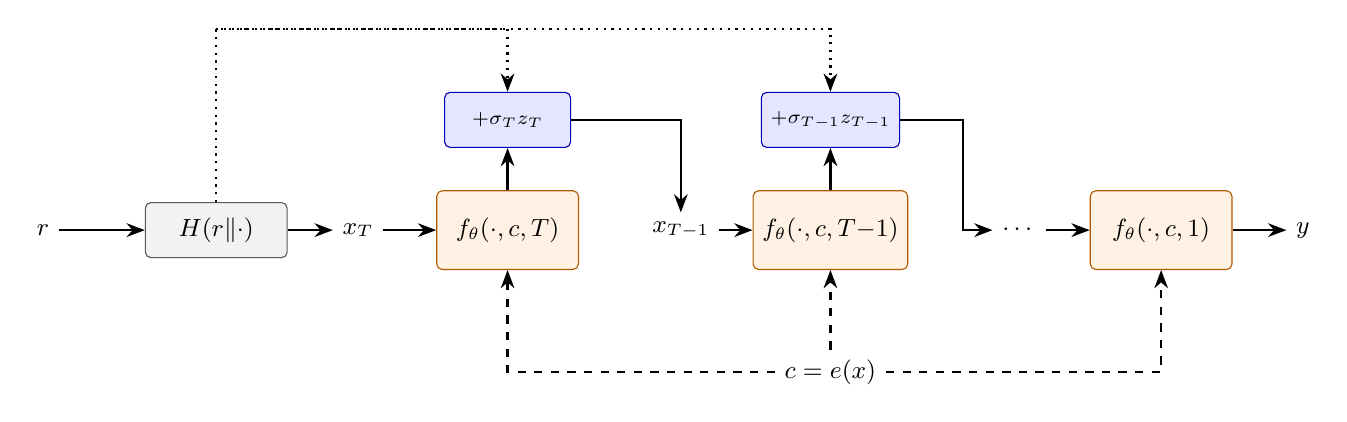
\begin{tikzpicture}[
    >=Stealth,
    font=\small,
    ubox/.style={draw=orange!70!black, rounded corners=2pt, minimum height=10mm,
                 minimum width=18mm, align=center, fill=orange!10, font=\small},
    nbox/.style={draw=blue!70!black, rounded corners=2pt, minimum height=7mm,
                 minimum width=16mm, align=center, fill=blue!10, font=\scriptsize},
    hbox/.style={draw=gray!70!black, rounded corners=2pt, minimum height=7mm,
                 minimum width=18mm, align=center, fill=gray!10, font=\scriptsize},
]
  % Inputs
  \node (r) at (-1.8,0) {$r$};
  \node[hbox, font=\small] (hash) at (0.4,0) {$H(r\|\cdot)$};
  % x_T
  \node (xT) at (2.2,0) {$x_T$};
  % Step T: UNet + noise
  \node[ubox] (u1) at (4.1,0) {$f_\theta(\cdot, c, T)$};
  \node[nbox] (n1) at (4.1,1.4) {$+\sigma_T z_T$};
  % x_{T-1}
  \node (xTm1) at (6.3,0) {$x_{T{-}1}$};
  % Step T-1: UNet + noise
  \node[ubox] (u1b) at (8.2,0) {$f_\theta(\cdot, c, T{-}1)$};
  \node[nbox] (n1b) at (8.2,1.4) {$+\sigma_{T{-}1} z_{T{-}1}$};
  % dots and final
  \node (dots) at (10.6,0) {$\cdots$};
  \node[ubox] (u2) at (12.4,0) {$f_\theta(\cdot, c, 1)$};
  \node (y) at (14.2,0) {$y$};
  % Conditioning
  \node (c) at (8.2,-1.8) {$c = e(x)$};
  % Main path arrows
  \draw[thick,->] (r) -- (hash);
  \draw[thick,->] (hash) -- (xT);
  \draw[thick,->] (xT) -- (u1);
  \draw[thick,->] (u1) -- (n1);
  \draw[thick,->] (n1.east) -| (xTm1.north);
  \draw[thick,->] (xTm1) -- (u1b);
  \draw[thick,->] (u1b) -- (n1b);
  \draw[thick,->] (n1b.east) -| ++(0.8,-1.4) -- (dots);
  \draw[thick,->] (dots) -- (u2);
  \draw[thick,->] (u2) -- (y);
  % Conditioning arrows
  \draw[thick,->,dashed] (c) -| (u1.south);
  \draw[thick,->,dashed] (c) -- (u1b.south);
  \draw[thick,->,dashed] (c) -| (u2.south);
  % Hash outputs for noise
  \draw[thick,->,dotted] (hash.north) -- ++(0,2.2) -| (n1.north);
  \draw[thick,->,dotted] (hash.north) ++(0,2.2) -| (n1b.north);
\end{tikzpicture}
\caption{Stochastic diffusion generation pipeline. A seed $r$ is expanded via a hash function $H$: the initial noise is $x_T = H(r\|0)$ and each per-step noise vector is $z_t = H(r\|T-t+1)$. Each denoising step applies $f_\theta$ (a neural network model) conditioned on $c = e(x)$ and adds scaled noise. The final step produces output $y$ without noise addition.}
\label{fig:diffusion-pipeline}
\end{figure*}

The denoising network $f_\theta$ is composed of standard neural network building blocks---convolutional layers, group normalisation, element-wise activations (SiLU/GeLU), self-attention and cross-attention layers, and residual connections---all arranged in a fixed architecture with predetermined layer dimensions.

\subsection{Cryptographic protocols}
\thomas{TODO asymmetric encryption, VRF add}
% This section reviews commitment schemes, zero-knowledge proofs (ZKPs), and multi-party computation (MPC). We use $\lambda$ as the security parameter and assume familiarity with computational indistinguishability and negligible functions $\negligible$.

\subsubsection{Commitment schemes}
\label{def: commitment}
Informally, a commitment scheme is a tuple $\Gamma = (\setup,\allowbreak \commit, \open)$ of $\ppt$ algorithms where: 
\begin{itemize} [itemsep=0em,nosep]
        \item $\setup(1^{\lambda}) \rightarrow \ppnew$ takes security parameter $\lambda$ and generates public parameters $\text{pp}$;
        \item $\commit(\ppnew; m) \rightarrow (\com,r)$ takes a secret message $m$, outputs a public commitment $Com$ and a randomness $r$ used in the commitment.
        \item $\open(\ppnew, \com; m, r) \rightarrow b \in \{0,1\}$ verifies the opening of the commitment $C$ to the message $m$ with the randomness $r$.
\end{itemize}

We require two main security properties: \emph{hiding} and \emph{binding}. Hiding ensures no $\ppt$ adversary can determine the committed message from $\com$. Binding ensures $\com$ can be opened to only one specific message. See App.~\ref{app:com} for formal definitions.

% \subsubsection{Merkle Tree Commitments}
% A Merkle tree commitment uses a collision-resistant hash function $H$ to commit to a vector $(m_1,$ $\ldots,$ $m_n)$ by hashing leaves and iteratively hashing pairs up a binary tree; the commitment is the root, and an opening is the $O(\log n)$-length authentication path for an index $i$.

% A merkle tree commitment is a tuple of PPT algorithms $\Gamma = (\mtsetup,\mtcommit,\mtopen,\mtverify)$ where:
% \begin{itemize}[leftmargin=1.25em]
%   \item $\mtsetup(1^\lambda)\to\ppnew$: generates public parameters $\ppnew$./
%   \item $\mtcommit(\ppnew; m_1,\ldots,m_n)\to(\com,\st)$: compute leaf and internal hashes; output root $\com$ and state $\st$.
%   \item $\mtopen(\ppnew,\st; i)\to\pi_i$: output the sibling-hash path authenticating position $i$.
%   \item $\mtverify(\ppnew,\com; i,m_i,\pi_i)\to b$: recompute the root from $(i,$ $m_i,$ $\pi_i)$ and accept iff it equals $\com$.
% \end{itemize}

% The position-binding property (no two different $m$ open at the same $i$) holds under collision resistance of $H$. We refer to App.~\ref{app:merkle} for the formal definition.


\subsubsection{Zero-knowledge proofs}
\label{def: NIZK}
A {\em non-interactive zero-knowledge proof-of-knowledge system (NIZKPoK)} for an \NP-language $L$ with the corresponding relation $\relation{L}$ is represented by a tuple of algorithms $\Pi = (\setup, \prover, \verifier)$, where:
    \begin{itemize}[itemsep=0em,nosep]
        \item $\setup( 1^{\lambda}) \rightarrow \crs$ takes as the input a security parameter $\lambda$. It outputs a common reference string $\crs$.
        \item $\prover(\crs, x, w) \rightarrow \pi$ takes as the input $\crs$, the statement $x$ and the witness $w$, s.t. $(x, w) \in \relation{L}$. It outputs the proof $\pi$.
        \item $\verifier(\crs, x, \pi) \rightarrow b \in \{0,1\}$ takes as the input $\crs$, $x$ and $\pi$. It outputs 1 to accept and 0 to reject.
    \end{itemize}

Informally, a NIZK proof is secure if it satisfies \emph{completeness}, \emph{zero-knowledge}, and \emph{soundness}. Completeness requires honest verifiers always accept honest proofs. Zero-knowledge ensures proofs leak no information about the witness $w$, even to malicious verifiers. Soundness requires verifiers reject proofs of false statements.
We refer to App.~\ref{app:zk} for the formal definition.


\subsection{Blockchain and Proof-of-Work Consensus}

A \emph{blockchain} is a decentralized, append-only ledger storing an ordered sequence of blocks; each block includes transactions, a timestamp, and the previous block's hash, yielding immutability~\cite{nakamoto2008bitcoin,bonneau2015sok}.

\subsubsection{Proof-of-Work Consensus}

In Proof-of-Work (PoW) consensus~\cite{nakamoto2008bitcoin}, miners compete to extend the blockchain by searching for a nonce $\mathit{ctr}$ such that $H(\mathit{ctr}, G(s, x)) < T$, where $H,G$ are cryptographic hash functions modelled as a random oracle, $s$ is the hash of the previous block, $x$ is the block content, and $T$ is a target threshold.  Because $H$ behaves as a random function, each query succeeds independently with probability $p = T/2^{\kappa}$, and the expected number of queries to produce a valid block is $1/p$.  The difficulty parameter $T$ is periodically adjusted so that blocks are produced at a target rate despite changes in the network's total hash power.

Garay, Kiayias, and Leonardos~\cite{GKL20} formalise Bitcoin's security in the \emph{backbone protocol} model under the assumption that each party makes at most $q$ random-oracle queries per round and that a strict honest majority of computational power is maintained. They establish three fundamental properties of the resulting longest-chain protocol---\emph{common prefix} (sufficiently deep blocks are agreed upon by all honest parties), \emph{chain quality} (a positive fraction of blocks in any window are honest), and \emph{chain growth} (honest chains grow at a predictable rate)---which together guarantee consistency and liveness. We state these properties formally in Section~\ref{sec:problem} and carry out our security reduction in Section~\ref{sec:reduction}. We refer the reader to~\cite{GKL20} and its variable-difficulty extension~\cite{GKL17} for the full formal treatment.
\section{Problem Description}
\label{sec:problem}
\begin{figure*}[t]
    \centering
    \includegraphics[width=0.8\textwidth]{plots/PoML.drawio.png}
    \caption{A high-level diagram of the proposed PoML blockchain. Users submit model queries to the mempool as pending requests. Model nodes retrieve these requests and compete to produce a valid block by executing model inference and generating zero-knowledge proofs attesting to correct execution. The first node to produce a valid block appends it to the blockchain and receives the associated rewards.}
    \label{fig:blockchain-poml}
\end{figure*}

We envision a blockchain architecture as illustrated in Figure~\ref{fig:blockchain-poml}. End users submit inference queries to the blockchain’s memory pool (mempool), where each query contains input data for which the user seeks a model inference result. Model nodes, also referred to as \emph{miners}, retrieve pending queries from the mempool and attempt to produce the next block by executing inference on the model and generating zero-knowledge proofs (ZKPs) attesting to the correctness of the computation. A miner successfully produces a block when it constructs what we refer to as a \emph{valid block}, containing verified inference outputs and coin transactions (not shown here for brevity), which is then appended to the blockchain in exchange for rewards.

The definition of a valid block lies at the core of our proposed Proof-of-ML-Inference (PoML) consensus mechanism and constitutes the central technical challenge of this work. The consensus protocol must be robust against adversarial behavior, ensuring that no participant can consistently produce valid blocks without honestly performing the required computation. This leads us to the following research question:

\noindent \emph{How can machine learning inference and the generation of corresponding zero-knowledge proofs be leveraged to design a robust and decentralized PoML consensus mechanism that achieves comparable security to Bitcoin's protocol?}

\subsection{The Model Class $\mathcal{K}$}
\label{subsec:model-class}

We define a class $\mathcal{K}$ of ML models suitable for use in PoML. Each model in $\mathcal{K}$ must satisfy two structural properties that we formalise below.

In Bitcoin, a hash function is modelled as a random oracle---any adversary learns $H(x)$ only by querying the oracle on $x$, and no shortcut exists. To achieve similar security in PoML, we require that model inference behaves analogously: the only way to obtain the output is to perform the full computation, with no shortcuts or precomputation.

We consider stochastic ML models $M_\theta$ parameterised by weights $\theta$ that accept two inputs: a \emph{conditioning input} $c$ (e.g., a text embedding produced by an encoder) and a \emph{random seed} $r \in \{0,1\}^\kappa$. Given both inputs, the model produces an output $y = M_\theta(c, r)$. The conditioning input captures the user's query, while the seed controls all stochasticity in the inference process.

\thomas{Michele, Rik: Tried my best to define this, I know it is not perfect. Can you see if it is ok, or how to change it?}

\begin{definition}[Uniform query cost]
\label{def:uniform-cost}
Let $\mathsf{Cost}(\cdot)$ be a function that counts the number of floating-point operations (FLOPs) of an evaluation. $M_\theta$ is said to have uniform query cost if for some fixed constant $k$, it satisfies $\mathsf{Cost}(M_\theta(c,r)) = k$ for all $(c, r)$.
\end{definition}

\begin{definition}[$\delta$-amortizability]
\label{def:delta-reuse}
Let $M_\theta$ be a model with uniform query cost and $\mathsf{Cost}(\cdot)$ be defined as above (Def~\ref{def:uniform-cost}). Assume $T_M:=\mathsf{Cost}(M_\theta)$ is the fixed cost of querying $M_\theta$ with no prior state. We say $M_\theta$ is \emph{$\delta$-amortizable} if for every probabilistic polynomial-time adversary $\mathcal{A}$, the following holds.

Consider the experiment $\textsf{Reuse}_{\mathcal{A}, M_\theta}(\kappa)$:
\begin{enumerate}
    \item \textbf{(Preprocessing)} $\mathcal{A}$ receives $\theta$ and may make polynomially many adaptive queries to $M_\theta(\cdot, \cdot)$, retaining arbitrary state $\textsf{st}$ (including any cached intermediate activations, partial computations, or precomputed lookup tables).
    \item \textbf{(Challenge)} A fresh seed is sampled: $r^* \leftarrow \{0,1\}^\kappa$, and $\mathcal{A}$ receives $r^*$.
    \item \textbf{(Evaluation)} $\mathcal{A}(\textsf{st}, r^*)$ selects $c^*$ and outputs $y^* = M_\theta(c^*, r^*)$.
\end{enumerate}

Let $T_{\mathcal{A}}:= \mathsf{Cost}(\mathcal{A}(\textsf{st}, r^*))$ denote the cost of step~3. Then:
\begin{equation}
    T_{\mathcal{A}} \geq (1 - \delta) \cdot T_M
\end{equation}
where $\delta \in [0, 1)$, with overwhelming probability. Informally, the adversary's prior evaluations and cached state grant at most a $\delta$-fraction speedup over a fresh evaluation.
\end{definition}


\begin{definition}[PoML-compatible model]
\label{def:model}
$M_\theta$ is said to be PoML-compatible if it has uniform query cost and is $\delta$-amortizable for a fixed $\delta$ in the PoML protocol. We denote $\mathcal{K}$ as the class of all PoML-compatible models.
\end{definition}

Intuitively, uniform query cost ensures that every inference incurs the same computational expense, preventing an adversary from cherry-picking cheap inputs. The $\delta$-amortizability property guarantees that distinct seeds produce distinct execution traces, so no intermediate computation from one inference can be reused for another, and there is no shortcut to performing each inference independently.

\subsubsection{Instantiation: Stochastic Denoising Models}
\label{subsec:diffusion-instantiation}

Stochastic denoising diffusion models (Section~\ref{subsec:diffusion-models}) are a natural instantiation of $\mathcal{K}$. They satisfy both properties of Definition~\ref{def:model}: \thomas{TODO check model definition clear enough?}
\begin{enumerate}
    \item \textbf{Uniform query cost.} The denoising network $f_\theta$ has a fixed architecture with predetermined layer dimensions, so each evaluation traverses an identical computational graph regardless of input values.
    \item \textbf{$\delta$-amortizability.} At each step $t \geq 2$, noise scaled by $\sigma_t > 0$ is injected into the denoiser output (eq.~\eqref{eq:ddpm-step-prelim}). Because distinct seeds produce independent noise vectors, intermediate states at every denoising step diverge across evaluations with overwhelming probability (Theorem~\ref{thm:cia-theorem}).
\end{enumerate}
The full argument that stochastic denoising models are PoML-compatible is given in Appendix~\ref{app:cia}.

\subsection{Solution Desiderata}

We require the PoML puzzle to satisfy properties that enable a formal security reduction to the Bitcoin backbone protocol~\cite{GKL20}. Concretely, our goal is to show that the PoML protocol inherits the three backbone guarantees established in~\cite{GKL20}:

\begin{description}[nosep]
\item[Common Prefix (CP).] For any parameter $k \in \mathbb{N}$, removing the last $k$ blocks from any honest party's chain yields a prefix of every other honest party's chain. This guarantees that sufficiently deep transactions are irrevocable.
\item[Chain Quality (CQ).] In any sufficiently long window of consecutive blocks on an honest party's chain, at least a fraction $\mu > 0$ were contributed by honest parties. This prevents an adversary from dominating the chain content.
\item[Chain Growth (CG).] The chain of any honest party grows by at least $\tau$ blocks per round (in expectation over sufficiently many rounds), ensuring liveness.
\end{description}

This reduction is carried out in Section~\ref{sec:reduction}. Informally, to achieve the three guarantees, the PoML puzzle must satisfy the following structural properties:

\begin{enumerate}
    \item \textbf{Grinding-resistance.} An adversary cannot cherry-pick model inputs to reduce inference and proof cost. 

    \item \textbf{Pre-computation resilience.} Problem instances cannot be manufactured or predicted in advance.

    \item \textbf{Amortisation-freeness.} Producing $k$ valid inference--proof pairs costs at least $k$ times the cost of a single pair. This is guaranteed by the $\delta$-amortizability property of the model class~$\mathcal{K}$ (Definition~\ref{def:delta-reuse}).
    
    \item \textbf{Adjustable difficulty.} The block difficulty is dynamically adjustable so that block time can be maintained as the network's aggregate computational power changes.

    \item \textbf{Efficient verification.} The running time of the verification algorithm is at most polylogarithmic in the prover's inference time.

    \item \textbf{Progress-freeness.} The probability of finding a valid block is independent of the computational effort already expended, ensuring mining is memoryless and preventing large miners from deterministically outpacing smaller ones.
\end{enumerate}

% \michele{it is not clear why we listed the above properties. Do we show that our puzzle satisfies them? }

% ---- OLD DESIDERATA (verbal, from Ali et al.) ----
% \begin{itemize}
%     \item \textbf{Asymmetry.}  
%     In the absence of trust between nodes, each node must independently verify the correctness of a solution. Verification should therefore be computationally inexpensive, while finding a solution should require substantial effort.
%
%     \item \textbf{Granularity and Parametrization.}  
%     As the network's computational power would scale with Moore's law, the difficulty of the puzzle should be dynamically adjustable to achieve desired network parameters, such as target block time.
%
%     \item \textbf{Amortization-Freeness.}  
%     Producing multiple valid solutions should incur a proportional increase in computational cost compared to producing a single solution.
%
%     \item \textbf{Independence.}  
%     Solving one instance of the puzzle should not provide any computational advantage when solving other instances.
%
%     \item \textbf{Unforgeability.}  
%     An adversary should not be able to construct puzzle instances that allow solutions to be precomputed in advance.
%
%     \item \textbf{Freshness.}  
%     A solution should not be valid indefinitely and cannot be used by other users.
%
%     \item \textbf{Progress-Freeness.}  
%     The probability of finding a solution should be independent of the effort already expended on the current instance.
%
%     \item \textbf{Public Verifiability.}  
%     Any party should be able to verify a solution non-interactively, without requiring participation from the prover.
% \end{itemize}


\section{The PoML Protocol}
\label{sec:protocol}

This section formally specifies the Proof-of-ML-Inference (PoML) consensus protocol. 

\subsection{System Model and Notation}
\label{sec:poml-system-def}

Let $\mathcal{N}$ denote the set of nodes (miners). Each node holds an identical model $M_\theta \in \mathcal{K}$ (Definition~\ref{def:model}) and a key pair $(\mathsf{pk}_m, \mathsf{sk}_m) \leftarrow \mathsf{KeyGen}_{\mathsf{pke}}(1^\kappa)$; we write $\mathcal{R}_{\mathsf{key}}$ for the induced key-pair relation, i.e., $(\mathsf{pk}_m, \mathsf{sk}_m) \in \mathcal{R}_{\mathsf{key}}$ iff $\mathsf{KeyGen}$ can output $(\mathsf{pk}_m, \mathsf{sk}_m)$. Since a public key may admit multiple valid secret keys, each node must also register a commitment to its secret key during registration:
\[
(c_{\mathsf{sk}},\, r_{\mathsf{sk}}) \leftarrow \mathsf{Commit}(\ppnew,\mathsf{sk}_m),
\]
and publish $c_{\mathsf{sk}}$ on-chain alongside~$\mathsf{pk}_m$. This binds the node to a unique secret key for the duration of its participation.

Let $\mathcal{U}$ denote the set of users submitting inference queries. Each user likewise holds a key pair $(\mathsf{pk}_u, \mathsf{sk}_u)$. A block is defined as $B = (s, x, \mathcal{X}, \mathcal{Y}, \Pi, \Pi^{(2)})$, where $s$ is the previous block hash, $x$ is the block content comprising standard coin transactions (transfers, fees, block rewards), $\mathcal{X}$ is the tuple of user queries to the model, $\mathcal{Y} = (\mathsf{ct}_1, \ldots, \mathsf{ct}_k)$ is the tuple of encrypted outputs, $\Pi = (\pi_1^{(1)}, \ldots, \pi_k^{(1)})$ and $\Pi^{(2)} = (\pi_1^{(2)}, \ldots, \pi_k^{(2)})$ ordered tuples of ZKPs which will be explained in the coming sections. 

We assume the following cryptographic primitives:
\begin{itemize}
    \item Commitment scheme: $(\mathsf{Setup}_\mathsf{com},\mathsf{Commit}, \open)$
  \item Hash function  $G,H : \{0,1\}^* \to \{0,1\}^\kappa$, used for seed derivation and the lottery
    \item Zero-knowledge proof systems $(\mathsf{Setup}_{\mathsf{zkp},1},\prover_1,\verifier_1)$, \\$(\mathsf{Setup}_{\mathsf{zkp},2},\prover_2,\verifier_2)$ for the two NP-languages described in the following sections
    \item Public-key encryption scheme $(\mathsf{KeyGen}_{\mathsf{pke}},\mathsf{Enc}, \mathsf{Dec})$
    \item Pseudorandom function $F : \{0,1\}^\kappa \times \{0,1\}^\kappa \to \{0,1\}^\kappa$, used to derive the prover's internal randomness 
    \item Digital signature scheme $(\mathsf{KeyGen}_{\mathsf{sig}}, \mathsf{Sign}, \mathsf{Verify}_{\mathsf{sig}})$
\end{itemize}

The public parameters $\mathsf{pp}$ and common reference string for the zero-knowledge proof $\mathsf{CRS}$ are assumed to be agreed out-of-band and published on the blockchain as parameters of the blockchain. The setup process for the commitment scheme and ZKP is also assumed to be done beforehand.

\subsection{Query Submission}

A user $u \in \mathcal{U}$ submits an inference request by providing a conditioning embedding $c = e(x)$, obtained by applying the public embedding function~$e$ to their input~$x$.

Each user maintains a running counter $\mathsf{taskID}$, which denotes the number of successful queries made. The user computes a commitment:
\begin{align}
    (\mathsf{c}_c, r_c) &\leftarrow \mathsf{Commit}(c \parallel \mathsf{taskID})
\end{align}

The user then signs and diffuses a query transaction to the network:
\[
\sigma_u \leftarrow \mathsf{Sign}(\mathsf{sk}_u,\, \mathsf{taskID} \parallel \mathsf{c}_c \parallel \text{fee}),
\]
\[
T_{\text{query}} = (\mathsf{pk}_u,\, \mathsf{taskID},\, \mathsf{c}_c,\, c,\, r_c,\, \text{fee},\, \sigma_u),
\]
where $\text{fee}$ is the cost of the query paid to the successful miner.
% The full transaction---including the embedding~$c$ and opening randomness~$r_c$---is diffused to the network so that miners can verify the commitment and perform inference. However, only the compact on-chain record
% \[
% \hat{T}_{\text{query}} = (\mathsf{pk}_u,\, \mathsf{taskID},\, \mathsf{c}_c,\, \text{fee},\, \sigma_u)
% \]
% is stored in the block. The embedding~$c$ and randomness~$r_c$ do not persist on-chain; the commitment~$\mathsf{c}_c$ suffices for proof verification.

\subsection{Query Retrieval}

Each node mines a block by retrieving queries from the mempool.

For each query, the miner verifies the user's signature \\$\mathsf{Verify}_{\mathsf{sig}}(\mathsf{pk}_u, \mathsf{taskID} \parallel \mathsf{c}_c \parallel \text{fee},\, \sigma_u) = 1$, checks the commitment opening $\open(\mathsf{pp}, \mathsf{c}_c, c \| \mathsf{taskID}, r_c) = 1$, and verifies that the $\mathsf{taskID}$ is correctly in order. If all checks pass, the miner proceeds with model inference.

\subsection{Inference and Proof Generation}

To build the block, miners first prepares the block content $G(s,x)$, then compute inferences and generate proofs one by one, forming a \textit{proof chain} $\Pi = (\pi_1^{(1)}, \ldots, \pi_k^{(1)})$. For the $i$-th query in the chain, the miner first derives a random seed:
\begin{equation}
r_i = H(G(s,x) \parallel \mathsf{c}_{c,i} \parallel \mathsf{taskID}_i \parallel \mathsf{pk}_m \parallel i),
\end{equation}
where $s$ is the previous block hash and $\mathsf{pk}_m$ is the miner's public key.

The model inference is computed as:
\begin{equation}
y_i = M_\theta(c_i, r_i).
\end{equation}

\paragraph{Output encryption and proof chain binding.}
Define the \emph{chain binding} for position~$i$ as:
\[
\mathsf{bind}_i = 
\begin{cases}
G(s,x) & \text{if } i = 1, \\
H(\pi_{i-1}^{(1)}) & \text{if } i \geq 2.
\end{cases}
\]
\thomas{Michele--We have to design the chain binding this way, cannot just use a position binding like H(1), H(2), otherwise this will break the proof-to-lottery bijection in section 5.3 - An adversary that e.g. runs two proofs in parallel for position 1 ($\pi_A^1,\pi_B^1$), two proofs in parallel for position 2 ($\pi_C^2,\pi_D^2$) can admit six different lottery chances ($\pi_A^1$),($\pi_A^1,\pi_C^2$), ($\pi_A^1,\pi_D^2$), ... for just four proofs}

The output is encrypted together with the chain binding and task ID under the querying user's public key:
\begin{align}
\label{eq:ct}
\mathsf{ct}_i \leftarrow \mathsf{Enc}(\mathsf{pk}_u,\, y_i \parallel \mathsf{bind}_i \parallel \mathsf{taskID}).
\end{align}

\paragraph{Proof statement.}
Nodes generate a zero-knowledge proof $\pi_i^{(1)}$ for membership in the NP language:

\[
\mathcal{L}_{\text{PoML}} 
= \left\{\,
  \begin{array}{@{}l@{}}
    (\mathsf{pp},\mathsf{taskID},\mathsf{bind}_i,\mathsf{c}_c,c_\theta, r_i, \mathsf{ct}_i, \mathsf{pk}_u):\\[0.2em]
    \exists\,(c,r_c,\theta,r_\theta,y) \ \text{s.t.} \\
    M_\theta(c, r_i)=y, \\
    \mathsf{Open}(\mathsf{pp},\mathsf{c}_c,c \,\|\, \mathsf{taskID},r_c) = 1, \\
    \mathsf{Open}(\mathsf{pp},c_\theta,\theta, r_\theta) = 1, \\
    \mathsf{ct}_i = \mathsf{Enc}(\mathsf{pk}_u,\, y \,\|\, \mathsf{bind}_i \,\|\, \mathsf{taskID})
  \end{array}
\right\}.
\]
We write $\mathsf{stmt}_i^{(1)} = (\mathsf{pp},\mathsf{taskID}_i,\mathsf{bind}_i,\mathsf{c}_{c,i},c_\theta, r_i, \mathsf{ct}_i, \mathsf{pk}_{u,i})$ for the public statement and $\mathsf{wit}_i^{(1)} = (c_i,r_{c,i},\theta,r_\theta,y_i)$ for the witness.

\paragraph{Deterministic proof generation.}
To prevent proof grinding---i.e., an adversary re-running the prover with different internal randomness to obtain distinct proofs for the same inference---we require that the prover's internal randomness is derived deterministically from the seed and the miner's secret key. Concretely, a pseudorandom function keyed by the miner's secret key expands the seed into prover randomness:
\[
\rho_i = F(\mathsf{sk}_m,\, r_i),
\]
and the miner generates the inference proof as \\ $\pi_i^{(1)} = \mathsf{Prove}(\mathsf{CRS},\, \mathsf{stmt}_i^{(1)},\, \mathsf{wit}_i^{(1)}\,;\; \rho_i)$, where $\rho_i$ replaces the prover's internal random tape. This ensures that each (miner, seed) pair $(\mathsf{sk}_m, r_i)$ yields a unique proof $\pi_i^{(1)}$, eliminating any advantage from re-randomization.

\paragraph{Meta-proof of deterministic proving.}
To enforce that the miner indeed used the prescribed randomness $\rho_i$, the miner additionally generates a \emph{meta-proof} $\pi_i^{(2)}$ for the language:
\[
\mathcal{L}_{\text{det}} = \left\{\,
  \begin{array}{@{}l@{}}
    (\mathsf{pp},\, r_i,\, \mathsf{stmt}_i^{(1)},\pi_i^{(1)},\, \mathsf{pk}_m,\, c_{\mathsf{sk}}):\\[0.2em]
    \exists\, (\mathsf{sk}_m,\, r_{\mathsf{sk}},\, \mathsf{wit}_i^{(1)}) \ \text{s.t.} \\
    (\mathsf{pk}_m, \mathsf{sk}_m) \in \mathcal{R}_{\mathsf{key}}, \\
    \mathsf{Open}(\mathsf{pp},\, c_{\mathsf{sk}},\, \mathsf{sk}_m,\, r_{\mathsf{sk}}) = 1, \\
    \rho_i = F(\mathsf{sk}_m,\, r_i), \\
    \pi_i^{(1)} = \mathsf{Prove}(\mathsf{CRS},\, \mathsf{stmt}_i^{(1)},\, \mathsf{wit}_i^{(1)}\,;\; \rho_i)
  \end{array}
\right\}.
\]
We write $\mathsf{stmt}_i^{(2)} = (\mathsf{pp}, r_i, \mathsf{stmt}_i^{(1)}, \pi_i^{(1)}, \mathsf{pk}_m, c_{\mathsf{sk}})$ for the public statement and $\mathsf{wit}_i^{(2)} = (\mathsf{sk}_m, r_{\mathsf{sk}}, \mathsf{wit}_i^{(1)})$ for the witness.
The meta-proof attests that $\pi_i^{(1)}$ was computed using the deterministic randomness $\rho_i = F(\mathsf{sk}_m, r_i)$, where $\mathsf{sk}_m$ is the miner's secret key corresponding to the public key~$\mathsf{pk}_m$ and matching the registered commitment~$c_{\mathsf{sk}}$. The zero-knowledge property of $\pi_i^{(2)}$ ensures that $\mathsf{sk}_m$ remains hidden. Each block therefore includes, for the $i$-th query, the pair $(\pi_i^{(1)}, \pi_i^{(2)})$.

\subsection{Block Construction and Consensus}

Nodes race to produce a valid block. To define a valid block, we introduce a lottery model which each node can run as soon as it has completed a proof within the block.

\paragraph{Lottery model.}

After generating proofs $\pi_i^{(1)}$ ($i \geq 1$), a lottery is executed based on the evolving block hash. Let $\Pi_i = (\pi_1^{(1)}, \ldots, \pi_i^{(1)})$ denote the inference proof tuple after the $i$-th proof. Since each proof $\pi_i^{(1)}$ is deterministically derived from the seed~$r_i$ (enforced by $\pi_i^{(2)}$), the lottery outcome is uniquely determined by the inference. We check:
\begin{equation}
H_i = H(G(s,x),\, \Pi_i) < D,
\end{equation} By adjusting $D$, we can tune the desired probability of lottery winning, hence the difficulty of the chain and other desired properties such as average block time.

If the above condition holds at any point, the miner can announce the block by publishing $B = (s, x, \mathcal{X}, \mathcal{Y}, \Pi, \Pi^{(2)})$. Each completed inference-proof pair yields exactly one lottery evaluation, motivating miners to process more queries and generate more proofs to increase their chance of winning.

\paragraph{Block validity.}

\begin{definition}[Valid Block]
\label{def:valid-block}
A block $B = (s,x,\mathcal{X}, \mathcal{Y}, \Pi, \Pi^{(2)})$ is valid,  iff the following conditions all hold:
\begin{enumerate}[nosep]
    \item \textbf{Lottery won:} $H(G(s,x),\, \Pi) < D$;
    \item \textbf{Non-empty proof tuples:} $|\mathcal{X}|=|\mathcal{Y}|=|\Pi|=|\Pi^{(2)}| \ge 1$;
    \item \textbf{Inference proofs verify:} $\mathsf{Verify}(\mathsf{CRS}, \mathsf{stmt}_i^{(1)}, \pi_i^{(1)}) = 1$ for all~$i$;
    \item \textbf{Meta-proofs verify:} $\mathsf{Verify}(\mathsf{CRS}, \mathsf{stmt}_i^{(2)}, \pi_i^{(2)}) = 1$ for all~$i$;
    \item \textbf{Transactions valid:} all coin transactions in $x$ are valid.
\end{enumerate}
\end{definition}

\subsection{Output Delivery}
\label{subsec:output-delivery}

In PoML, inference outputs are delivered privately to the querying user via public-key encryption. For each completed inference $y_i$, the miner encrypts the output under the user's public key (eq.\ref{eq:ct})
and includes the ciphertext $\mathsf{ct}_i$ in the encrypted-output tuple~$\mathcal{Y}$ of the block. Upon receiving the published block, the user decrypts the output using their secret key: $y_i \parallel \mathsf{bind}_i \parallel \mathsf{taskID} = \mathsf{Dec}(\mathsf{sk}_u,\, \mathsf{ct}_i)$. 

\subsection{Consensus Algorithm}

Algorithm~\ref{alg:poml-main} summarises the PoML block production procedure.

The protocol follows the longest-chain rule: upon receiving a new valid block, each node verifies all five conditions in Definition~\ref{def:valid-block} and adopts the longest valid chain. Ties are broken by the first block received.

\begin{algorithm}[t]
\caption{PoML Block Production}
\label{alg:poml-main}
\begin{algorithmic}[1]
\Require $B_{\mathsf{prev}}$ (previous block), $D$ (difficulty threshold), $\mathsf{CRS}$, $\mathsf{pp}$, $(\mathsf{pk}_m, \mathsf{sk}_m)$, $c_{\mathsf{sk}}$, $M_\theta$, $c_\theta$, $F$, $G$, $H$ as defined in \S\ref{sec:poml-system-def}
\State Retrieve query transactions from mempool; assemble block content~$x$
\State Initialize $s \gets H(B_{\mathsf{prev}})$, $\Pi \gets ()$, $\Pi^{(2)} \gets ()$, $\mathcal{X} \gets ()$, $\mathcal{Y} \gets ()$, $i \gets 0$
\Repeat
    \State $i \gets i + 1$
    \State Select next query 
    \Statex \qquad $T_i := (\mathsf{pk}_{u,i}, \mathsf{taskID}_i, \mathsf{c}_{c,i}, c_i, r_{c,i}, \text{fee}_i, \sigma_{u,i})$ 
    \Statex \qquad from the mempool
    \State Verify signature:
    \Statex \qquad $\mathsf{Verify}_{\mathsf{sig}}(\mathsf{pk}_{u,i},\, \mathsf{taskID}_i \| \mathsf{c}_{c,i} \| \text{fee}_i,\, \sigma_{u,i}) = 1$
    \State Verify commitment opening:
    \Statex \qquad $\open(\mathsf{pp},\, \mathsf{c}_{c,i},\, c_i \| \mathsf{taskID}_i,\, r_{c,i}) = 1$
    \State Derive seed $r_i \gets H(G(s,x) \parallel \mathsf{c}_{c,i} \parallel \mathsf{taskID}_i \parallel \mathsf{pk}_m \parallel i)$
    \State Compute inference $y_i \gets M_\theta(c_i, r_i)$
    \State Encrypt output $\mathsf{ct}_i \gets \mathsf{Enc}(\mathsf{pk}_{u,i},\, y_i \parallel \mathsf{bind}_i \parallel \mathsf{taskID}_i)$
    \State Derive prover randomness $\rho_i \gets F(\mathsf{sk}_m, r_i)$
    \State Generate inference proof:
    \Statex \qquad $\pi_i^{(1)} \gets \mathsf{Prove}(\mathsf{CRS},\, \mathsf{stmt}_i^{(1)},\, \mathsf{wit}_i^{(1)}\,;\; \rho_i)$
    \State Generate meta-proof:
    \Statex \qquad $\pi_i^{(2)} \gets \mathsf{Prove}(\mathsf{CRS},\, \mathsf{stmt}_i^{(2)},\, \mathsf{wit}_i^{(2)})$
    \State $\Pi \gets \Pi \,\|\, \pi_i^{(1)}$; $\Pi^{(2)} \gets \Pi^{(2)} \,\|\, \pi_i^{(2)}$; 
    \Statex \qquad $\mathcal{X} \gets \mathcal{X} \,\|\, \hat{T}_i$; $\mathcal{Y} \gets \mathcal{Y} \,\|\, \mathsf{ct}_i$
    \Statex \qquad \textit{// $\hat{T}_i = (\mathsf{pk}_{u,i}, \mathsf{taskID}_i, \mathsf{c}_{c,i}, \text{fee}_i, \sigma_{u,i})$ is the compact on-chain record}
    \State Compute $H_i \gets H(G(s,x),\, \Pi)$
\Until{$H_i < D$}
\State \textbf{Publish} block $B = (s, x, \mathcal{X}, \mathcal{Y}, \Pi, \Pi^{(2)})$
\end{algorithmic}
\end{algorithm}
\section{Security Reduction: PoML to the Bitcoin Backbone} 
\label{sec:reduction}

In this section, we formally show that the PoML consensus mechanism inherits the fundamental security properties established by Garay, Kiayias, and Leonardos~\cite{GKL20} for the Bitcoin backbone protocol---namely \emph{common prefix}, \emph{chain quality}, and \emph{chain growth}.

The central idea is to show that the \emph{composite operation} of ML inference, proof generation, and hash evaluation plays the same structural role in PoML that the random oracle~$H$ plays in Bitcoin. In Bitcoin, the only way to obtain a lottery ticket (a potential valid block) is to query the random oracle; no shortcut exists. In PoML, we establish an analogous property: the only way to obtain a lottery ticket is to execute the full pipeline of inference, proof, and hash evaluation---effectively querying an \emph{inference oracle}. Once this correspondence is in place, the backbone's $q$-bounded random oracle framework applies directly, and all three backbone guarantees carry over with suitably adjusted parameters.

We adopt the notation of~\cite{GKL20} throughout (cf.\ Table~1 therein). In particular:
\begin{itemize}
    \item $\kappa$: the security parameter and length of the hash function output (i.e., $H : \{0,1\}^* \to \{0,1\}^\kappa$);
    \item $\lambda$: the tail-bounds parameter, i.e., the minimum number of consecutive rounds over which concentration of the random variables $X$, $Y$, $Z$ is required (cf.\ Definition~9 in~\cite{GKL20}), with $\lambda \geq 2/f$;
    \item $n$: total number of parties (miners), of which $t$ are controlled by the adversary;
    \item $\gamma$: honest majority slack, $t/(n-t) \leq 1 - \gamma$ (denoted $\delta$ in~\cite{GKL20}; we reserve $\delta$ for the amortizability parameter of Definition~\ref{def:delta-reuse});
    \item $f$: probability that at least one honest party succeeds in finding a PoW in a round;
    \item $\varepsilon \in (0,1)$: quality of concentration of random variables in typical executions;
    \item $L$: total runtime of the system (in rounds);
    \item $Q = qnL$: total number of random oracle queries;
    \item $\mathcal{C}^{\lceil k}$: the chain obtained by removing the last $k$ blocks from $\mathcal{C}$; $\mathcal{C}_1 \preceq \mathcal{C}_2$ denotes that $\mathcal{C}_1$ is a prefix of $\mathcal{C}_2$.
\end{itemize}


\subsection{Reduction Framework}

Recall that the backbone protocol operates in rounds, with $n$ parties of which at most $t$ are corrupted. A \textit{block} is defined in the form $B = (s,x,ctr)$, where $s$ is the previous block hash, $x$ is the block content, and $ctr$ is a counter of queries to the random oracle $H$. $B$ should satisfy the $\mathsf{validblock}^T_q$ predicate, defined as
\[
(H(ctr,G(s,x))<T) \wedge (ctr \leq q).
\]
Crucially, each flat-model party (i.e. party with same amount of computational resource assumed) is limited to $q$ queries to the random oracle per round, and the only way to produce a valid block is to query this oracle---there is no shortcut.

In PoML, the role of the random oracle is replaced by an \emph{inference oracle}: each completed ML inference coupled with a valid ZKP and a hash evaluation constitutes one query to this oracle, yielding one ``lottery ticket.''  We denote by $q_{\mathsf{ML}}$ the maximum number of such oracle queries a single flat-model honest party can complete per round, and by $D$ the PoML difficulty parameter (the lottery threshold, i.e., a block candidate is valid if $H_i < D$). We define a block in PoML as $B = (s, x, \mathcal{X}, \mathcal{Y}, \Pi, \Pi^{(2)})$.  Our $\mathsf{validblock}^D_{q_{\mathsf{ML}}}$ predicate is defined as:
\[
\begin{aligned}
(& H(G(s,x), \Pi) < D) \\
\wedge\;& (1 \le |\mathcal{X}| = |\mathcal{Y}| = |\Pi| = |\Pi^{(2)}| \le q_{\mathsf{ML}}) \\
\wedge\;& (\forall i,\ 
\mathsf{Verify}(\mathsf{CRS},\mathsf{stmt}_i^{(1)},\pi_i^{(1)})=1 ) \\
\wedge\;& (\forall i,\ 
\mathsf{Verify}(\mathsf{CRS},\mathsf{stmt}_i^{(2)},\pi_i^{(2)})=1 ).
\end{aligned}
\]


We now show that this mechanism can be mapped into the backbone's $q$-bounded framework---with the inference oracle taking the place of the random oracle---and thus inherits all its properties.

Our reduction proceeds in five steps:
\begin{enumerate}[nosep]
    \item Bound the number of inference-proof pairs per round to $q_{\mathsf{ML}}$ via amortisation resistance.
    \item Establish a bijection between proof tuples and lottery evaluations.
    \item Establish that the PoML lottery is a $q_{\mathsf{ML}}$-bounded \emph{inference oracle}.
    \item Derive the success probability $f$ for PoML.
    \item Verify typicality of executions.
\end{enumerate}

\subsection{Step 1: Bounding Inference-Proof Pairs}
\label{subsec:step0}

In Bitcoin's backbone protocol, security relies on the assumption that each flat-model party can make at most $q$ queries per round to the random oracle $H$. This bound assumes the uniform cost of each hash evaluation.

In PoML, the analogous bound must hold for \emph{inference-proof pairs}: each pair consists of (i) a model inference $M_\theta(c,r)$ and (ii) the corresponding ZKP $\pi^{(1)}$. Recall from Section~\ref{subsec:model-class} that the model class $\mathcal{K}$ consists of models with \emph{uniform query cost} (Definition~\ref{def:uniform-cost}) and \emph{$\delta$-amortizability} (Definition~\ref{def:delta-reuse}). We show that both the inference and proof generation components inherit $\delta$-amortizability, bounding the number of inference-proof pairs per round to $q_\mathsf{ML}$.

\begin{theorem}[$q_{\mathsf{ML}}$-bounded inference-proof pairs]
\label{thm:amort-resist}
Let $M_\theta \in \mathcal{K}$ be a PoML-compatible model (Definition~\ref{def:model}) with $\delta$-amortizability parameter satisfying
\begin{equation}\label{eq:delta-bound}
    \delta \;<\; \frac{1}{q_{\mathsf{ML}} + 1},
\end{equation}
and let the proof system be a non-interactive zk-SNARK. Then, in every round, each flat-model party can complete at most $q_{\mathsf{ML}}$ inference-proof pairs, except with negligible probability in $\kappa$.
\end{theorem}

\begin{proof}
Let $T_M^{\mathsf{inf}}$ and $T_M^{\mathsf{pf}}$ denote the cost of a single model inference and a single proof generation, respectively, and let $T_M = T_M^{\mathsf{inf}} + T_M^{\mathsf{pf}}$ be the cost per inference-proof pair. Let $T_{\mathsf{round}}$ denote the computation budget of a flat-model party per round, so the honest count is $q_{\mathsf{ML}} = \lfloor T_{\mathsf{round}} / T_M \rfloor$ pairs.

\paragraph{Inference cost.}
 By Definition~\ref{def:delta-reuse}, any PPT adversary requires at least $(1-\delta) \cdot T_M^{\mathsf{inf}}$ cost per inference, regardless of preprocessing or cached state.

\paragraph{Proof generation cost.}
In a non-interactive zk-SNARK, the prover's computation is a deterministic function of the common reference string (CRS), the witness, and the Fiat--Shamir challenges derived from the transcript. The witness for pair~$i$ consists of all intermediate wire values of $M_\theta(c_i, r_i)$, which by the $\delta$-amortizability of~$\mathcal{K}$ differ from those of any prior pair in at least a $(1-\delta)$-fraction of entries, with overwhelming probability. Since the prover's per-constraint computation depends on the witness values at that constraint, at most a $\delta$-fraction of the prover's work can be reused across pairs. Therefore proof generation is also $\delta$-amortizable: any adversary requires at least $(1-\delta) \cdot T_M^{\mathsf{pf}}$ per proof.

\paragraph{Combined bound.}
The adversary's per-pair cost is at least $(1-\delta) \cdot T_M^{\mathsf{inf}} + (1-\delta) \cdot T_M^{\mathsf{pf}} = (1-\delta) \cdot T_M$, yielding at most
\[
    \left\lfloor \frac{T_{\mathsf{round}}}{(1-\delta) \cdot T_M} \right\rfloor 
    = \left\lfloor \frac{q_{\mathsf{ML}}}{1 - \delta} \right\rfloor
\]
pairs. Under condition~\eqref{eq:delta-bound}, $q_{\mathsf{ML}} / (1-\delta) < q_{\mathsf{ML}} + 1$, so the floor equals $q_{\mathsf{ML}}$ and the adversary gains no additional inference-proof pair.
\end{proof}

In practical PoML deployments where $q_{\mathsf{ML}}$ is small, the bound~\eqref{eq:delta-bound} on $\delta$ is not prohibitively tight. That stochastic denoising models satisfy $\delta$-amortizability with $\delta = \mathsf{negl}(\kappa)$ is established in Appendix~\ref{app:cia}.


\subsection{Step 2: Proof-to-Lottery Bijection}

In Step~1, we established that each flat-model party can produce at most $q_{\mathsf{ML}}$ inference-proof pairs per round. However, the lottery evaluation $H(G(s,x), \Pi_i)$ is a single hash---computationally negligible compared to inference and proof generation. Thus, the security-relevant question is whether an adversary can construct \emph{additional valid proof tuples} $\Pi$ from its $q_{\mathsf{ML}}$ inference-proof pairs, thereby extracting extra lottery evaluations without extra inference work. In Bitcoin, this step is trivial: each hash query $H(\mathit{ctr}, G(s,x))$ yields exactly one lottery ticket, and distinct counters give independent evaluations. In PoML, we must rule out that an adversary could obtain additional lottery tickets by reordering proofs, reusing proofs across blocks, forging proofs, or re-randomizing proofs.

\begin{lemma}[Proof-to-Lottery Bijection]\label{lem:bijection}
Let each party complete at most $q_{\mathsf{ML}}$ inference-proof pairs per round, with each proof generated using deterministic prover randomness enforced by the meta-proof $\pi_i^{(2)}$. Then each party can construct at most $q_{\mathsf{ML}}$ distinct valid proof tuples $\Pi$, and consequently obtains at most $q_{\mathsf{ML}}$ lottery evaluations per round. In particular, no adversary can obtain more than $t \cdot q_{\mathsf{ML}}$ lottery evaluations per round across all its controlled parties.
\end{lemma}

\begin{proof}
Fix a miner $(\mathsf{pk}_m, c_{\mathsf{sk}})$ and block header $(s, x)$. We prove by induction on the number of proofs~$k$ the adversary has generated that the set of valid proof tuples has cardinality at most~$k$, except with negligible probability. 

We first establish a key uniqueness property used throughout the induction.

\paragraph{Proof uniqueness.}
For a given inference $M_\theta(c_j, r_j)$ and chain binding $\mathsf{bind}$, there exists at most one valid proof $\pi_j^{(1)}$ with a valid meta-proof $\pi_j^{(2)}$. Indeed, the deterministic randomness $\rho_j = F(\mathsf{sk}_m, r_j)$ fixes $\pi_j^{(1)} = \mathsf{Prove}(\mathsf{CRS},\, \mathsf{stmt}_j^{(1)},\, \mathsf{wit}_j^{(1)}\,;\; \rho_j)$ uniquely. Any alternative $\tilde{\pi} \neq \pi_j^{(1)}$ would require either a valid proof for an incorrect witness (contradicting ZKP soundness), the use of different randomness (contradicting meta-proof soundness), a different block binding (contradicting collision resistance of~$G$), or originating from a different miner (contradicting PRF security and binding of~$c_{\mathsf{sk}}$)---each negligible in $\kappa$.

\paragraph{Base case $(k = 1)$.}
The adversary generates its first proof~$\pi^*$, which has a chain binding $\mathsf{bind}_1 = G(s,x)$ (position 1) baked into its ZKP statement. This creates exactly one valid tuple $(\pi^*)$. By the uniqueness property, no alternative proof $\tilde{\pi} \neq \pi^*$ can form a valid length-1 tuple. Hence there is exactly one valid proof tuple.

\paragraph{Inductive step.}
Assume that after $k$ proofs, the adversary has produced at most $k$ distinct valid proof tuples. Let $\mathcal{S}_k$ denote this set. The adversary generates the $(k+1)$-th proof $\pi^*$. We show that $|\mathcal{S}_{k+1}| \leq k + 1$ by analyzing where $\pi^*$ is bound.

\emph{Case 1: $\pi^*$ is at position $1$} (bound to $G(s,x)$). The new proof forms a length-1 tuple $(\pi^*)$. This is the only new tuple: any longer tuple containing $\pi^*$ as its first element would need a proof at position~2 with binding $H(\pi^*)$. No previously generated proof can have this binding, since producing such a proof before $\pi^*$ exists would require predicting $H(\pi^*)$---a hash preimage, infeasible except with negligible probability. Hence $\pi^*$ contributes exactly one new tuple: $|\mathcal{S}_{k+1}| \leq k + 1$.

\emph{Case 2: $\pi^*$ is at position $i \geq 2$} (bound to $H(\pi_{\mathrm{prev}})$ for some existing proof $\pi_{\mathrm{prev}}$). The binding $\mathsf{bind}_i = H(\pi_{\mathrm{prev}})$ uniquely identifies the predecessor $\pi_{\mathrm{prev}}$ by collision resistance of~$H$. We first argue that all tuples in $\mathcal{S}_k$ containing $\pi_{\mathrm{prev}}$ share the same prefix up to~$\pi_{\mathrm{prev}}$. Indeed, the chain binding of $\pi_{\mathrm{prev}}$ determines its predecessor $\pi_{\mathrm{prev}-1}$, which in turn determines $\pi_{\mathrm{prev}-2}$, and so on back to $G(s,x)$. Therefore, there is a unique chain $\Pi_{\mathrm{prev}} = (\pi_1, \ldots, \pi_{\mathrm{prev}})$ from the root to $\pi_{\mathrm{prev}}$, and the new proof~$\pi^*$ extends it to exactly one new tuple $\Pi_{\mathrm{prev}} \| (\pi^*)$. Since $\pi^*$ is unique for its binding (by the proof uniqueness property), no other extension of this prefix is possible. Hence $|\mathcal{S}_{k+1}| \leq k + 1$.

\paragraph{Conclusion.}
In all cases, each new proof increases the number of valid proof tuples by at most one. After $q_{\mathsf{ML}}$ proofs, there are at most $q_{\mathsf{ML}}$ valid tuples, each yielding one lottery evaluation $H(G(s,x), \Pi)$. Since each corrupted party faces the same constraint, an adversary controlling $t$ parties obtains at most $t \cdot q_{\mathsf{ML}}$ lottery evaluations per round.
\end{proof}

% \begin{remark}[Sequentiality of proof chains]
% The proof chain $(\pi_1, \ldots, \pi_i)$ is sequential: proof $\pi_i$ must be completed before lottery ticket $i$ can be evaluated, since $H_i$ depends on all preceding proofs. Unlike PoW where nonce attempts within a round are parallelizable, a PoML miner cannot ``skip ahead'' to later lottery tickets. However, this sequential structure does \emph{not} expand the adversary's strategy space: the total number of lottery tickets per round remains bounded by $t \cdot q_{\mathsf{ML}}$, exactly as in the backbone's $q$-bounded model. The adversary's only strategic choice is \emph{how to allocate} its $t \cdot q_{\mathsf{ML}}$ proof completions across candidate blocks---a form of selective publishing already captured in the backbone analysis.
% \end{remark}

\subsection{Step 3: The PoML Lottery as a $q_\mathsf{ML}$-Bounded Oracle}

Steps~1 and~2 together show that each flat-model party can produce at most $q_{\mathsf{ML}}$ inference-proof pairs per round (Theorem~\ref{thm:amort-resist}), and that each pair yields exactly one lottery evaluation (Lemma~\ref{lem:bijection}). We now combine these results: define an \emph{inference oracle} as the full pipeline of inference, proof, and hash evaluation on one user inference request. Each party makes at most $q_{\mathsf{ML}}$ queries to this oracle per round. Since the lottery outcome is determined by $H$ (a random oracle), the statistical properties of the PoML lottery are identical to those of Bitcoin's $q$-bounded random oracle.

\begin{lemma}[PoML lottery equivalence]
\label{lem:lottery-equiv}
Under the random oracle model for $H(\cdot)$, the PoML lottery mechanism (Definition~\ref{def:valid-block}) is equivalent to Bitcoin's $q$-bounded random oracle for block validity.
\end{lemma}

\begin{proof}
By Lemma~\ref{lem:bijection}, each party obtains exactly $q_{\mathsf{ML}}$ queries to the inference oracle. Each query evaluates $H_i = H(G(s,x), \Pi)$ and checks $H_i < D$. Since $H$ is modeled as a random oracle with output in $\{0,1\}^\kappa$, each evaluation $H_i$ produces an output uniformly distributed over $\{0,1\}^\kappa$, independent of all previous queries. The per-query success probability is:
\[
    p = \Pr[H(G(s,x), \Pi) < D] = \frac{D}{2^{\kappa}}.
\]
Therefore, each party makes at most $q_{\mathsf{ML}}$ independent random oracle queries per round, each succeeding with probability $p$.

This is structurally identical to the backbone's PoW mechanism where each party makes at most $q$ queries per round to $H$, each succeeding with probability $T / 2^\kappa$. The mapping is:
\[
    q \mapsto q_{\mathsf{ML}}, \qquad T \mapsto D.
\]
\end{proof}


\subsection{Step 4: Deriving $f$ for PoML}

The backbone analysis defines $f$ as the probability that at least one honest party obtains a valid block in a given round. By Lemma~\ref{lem:lottery-equiv}, each of the $(n - t)$ honest parties makes $q_{\mathsf{ML}}$ independent random oracle queries per round, each succeeding with probability $p = D / 2^\kappa$. Therefore:

\[
    f = 1 - (1 - p)^{(n-t) \cdot q_{\mathsf{ML}}}.
\]

For small $p \cdot (n-t) \cdot q_{\mathsf{ML}}$, this approximates to:
\[
    f \approx (n - t) \cdot q_{\mathsf{ML}} \cdot \frac{D}{2^\kappa}.
\]

Since $q_{\mathsf{ML}} \ll q$ (ML inference is orders of magnitude slower than hash computation), the resulting $f$ is naturally smaller for PoML than for PoW at equivalent network sizes. That said, the difficulty parameter $D$ still can be tuned to achieve any desired $f$. For a target block time of $\tau$ seconds with rounds of duration $\Delta$ seconds:
% A smaller $f$ is \emph{favorable} for security: it increases the ratio of uniquely successful rounds ($Y_i = 1$) relative to multiply successful rounds, tightening the bound in Lemma~11 of~\cite{GKL20}. Concretely, the probability that a round is uniquely successful given it is successful approaches~1 as $f \to 0$:
% \[
%     \Pr[Y_i = 1 \mid X_i = 1] = \frac{(n-t) \cdot q_{\mathsf{ML}} \cdot p \cdot (1-p)^{(n-t) \cdot q_{\mathsf{ML}} - 1}}{f}
% \]
% \[
%     \to 1 \quad \text{as } f \to 0.
% \]

%TODO remark 3 of 


\[
    D = \frac{f \cdot 2^\kappa}{(n - t) \cdot q_{\mathsf{ML}}}, \qquad \text{where } f = \frac{\Delta}{\tau}.
\]

% \begin{remark}
% The condition~\eqref{eq:honest-majority} is easier to satisfy in PoML than in PoW precisely because $f$ is smaller. This means PoML can tolerate adversarial fractions closer to $1/2$ for the same network synchronicity assumptions.
% \end{remark}

\subsection{Step 5: Typicality of Executions}

The backbone's security proofs operate within the ``typical execution'' framework (Definition~9, Theorem~10 in~\cite{GKL20}). An execution is \emph{$(\varepsilon, \lambda)$-typical} if, for any set $S$ of at least $\lambda$ consecutive rounds (where $\lambda \geq 2/f$), the following hold:
\begin{enumerate}
    \item[(a)] $(1 - \varepsilon)\mathbb{E}[X(S)] < X(S) < (1 + \varepsilon)\mathbb{E}[X(S)]$ \text{and} \\ $(1 - \varepsilon)\mathbb{E}[Y(S)] < Y(S)$.
    \item[(b)] $Z(S) < \mathbb{E}[Z(S)] + \varepsilon \mathbb{E}[X(S)]$.
    \item[(c)] No insertions, no copies, and no predictions occurred.
\end{enumerate}

Here $X(S) = \sum_{r \in S} X_r$ counts the number of \emph{successful} rounds in $S$ (rounds in which at least one honest party obtains a valid block), $Y(S) = \sum_{r \in S} Y_r$ counts the number of \emph{uniquely successful} rounds (exactly one honest party succeeds), and $Z(S) = \sum_{r \in S} Z_r$ counts the number of rounds in which at least one adversarial party succeeds. In PoML, we adopt the exact same definitions.

\begin{lemma}[Typicality under PoML]
\label{lem:typicality}
PoML executions are $(\varepsilon, \lambda)$-typical (Definition~9 in~\cite{GKL20}) with probability at least
$1 - e^{-\Omega(\varepsilon^2 f \lambda \;+\; \kappa \;-\; \log L)}$.
\end{lemma}

\begin{proof}
By Lemma~\ref{lem:lottery-equiv}, the PoML lottery operates in the $q_{\mathsf{ML}}$-bounded random oracle model with the \emph{same} random oracle $H$ as the backbone protocol. In particular, each lottery query evaluates $H$ on a distinct input (due to the sequentially-bound proof chain), and each evaluation succeeds independently with probability $D/2^\kappa$. This is structurally identical to the backbone's PoW lottery: independent Bernoulli trials under a $q$-bounded random oracle.  Therefore, the random variables $X_r, Y_r, Z_r$ in PoML satisfy the same independence and distributional properties as in the backbone, and the proof of Theorem~10 in~\cite{GKL20} (Chernoff bounds for parts (a)--(b), collision/prediction bounds for part (c)) applies verbatim with $q = q_{\mathsf{ML}}$ and $T = D$.
\end{proof}
% (Note that although PoML evaluations within a round are \emph{sequential}---unlike Bitcoin's parallelizable hash queries---this affects only computation time, not the statistical properties: the Chernoff bounds require independence, not parallelizability, and independence follows from the random oracle model.)

% \begin{remark}
% \red{For the overall probability to be negligible, we need $\varepsilon^2 f \lambda \gg \log L$ . Since $f$ is small (fewer lottery tickets per round), we would require a larger $\lambda$ to compensate. In words: PoML needs longer observation windows before the security guarantees take effect.}
% \end{remark}

% \begin{remark}[Variable inference time]
% In practice, the number of completed inferences per round may vary due to hardware heterogeneity or model complexity. If $q_{\mathsf{ML}}$ is not deterministic but is instead a random variable with bounded support $[q_{\min}, q_{\max}]$, the concentration bounds still hold by conditioning on the worst case $q_{\mathsf{ML}} = q_{\max}$ for the adversary and $q_{\mathsf{ML}} = q_{\min}$ for honest parties. The honest majority condition~\eqref{eq:honest-majority} must then be verified under these worst-case assumptions:
% \[
%     t \cdot q_{\max} < (1 - \gamma) \cdot (n - t) \cdot q_{\min}.
% \]
% This is a strictly stronger requirement than the flat-model assumption, but is necessary to account for hardware variance in practice.
% \end{remark}

\subsection{Main Theorem}

Combining the above results, we obtain the following:

\begin{theorem}[PoML inherits backbone properties]
\label{thm:main-reduction}
Let $\Pi_{\mathsf{PoML}}$ denote the PoML consensus protocol with $n$ parties, at most $t$ of which are corrupted. Each party can complete at most $q_{\mathsf{ML}}$ inference-proof pairs per round. Let $\kappa$ denote the security parameter (hash output length) and $\lambda \geq 2/f$ the tail-bounds parameter. Suppose the model's amortizability parameter satisfies $\delta < 1/(q_{\mathsf{ML}} + 1)$ (Theorem~\ref{thm:amort-resist}). Define:
\[
    f = 1 - (1 - D / 2^\kappa)^{(n-t) \cdot q_{\mathsf{ML}}}.
\]

If the honest majority condition
\[
    t \leq (1 - \gamma)(n - t), \qquad 3f + 3\varepsilon < \gamma,
\]
is satisfied, then $\Pi_{\mathsf{PoML}}$ satisfies the following properties for any $(\varepsilon, \lambda)$-typical execution (which occurs with probability at least $1 - e^{-\Omega(\varepsilon^2 f \lambda \;+\; \kappa \;-\; \log L)}$):
\begin{enumerate}
    \item \textbf{Common Prefix} with parameter $k \geq 2\lambda f$: for any two honest parties with chains $\mathcal{C}_1$, $\mathcal{C}_2$ adopted at rounds $r_1 \leq r_2$, $\mathcal{C}_1^{\lceil k} \preceq \mathcal{C}_2$.
    \item \textbf{Chain Quality} with parameters $\mu$ and $\ell \geq 2\lambda f$: in any $\ell$ consecutive blocks of any honest party's chain, the fraction of honest blocks is at least $\mu$, where $\mu \geq 1 - (1 + \frac{\gamma}{2}) \frac{t}{n - t} \cdot \frac{1}{1 - \gamma}$.
    \item \textbf{Chain Growth} with parameters $\tau$ and $s$: for any $s \geq \lambda$ consecutive rounds, the chain of any honest party grows by at least $\tau \cdot s$ blocks, where $\tau = (1 - \varepsilon)f$.
\end{enumerate}
\end{theorem}

\begin{proof}
By Lemma~\ref{lem:bijection}, each party's $q_{\mathsf{ML}}$ inference-proof completions yield exactly $q_{\mathsf{ML}}$ lottery queries to the random oracle, and the adversary is bounded to $t \cdot q_{\mathsf{ML}}$ queries per round. By Lemma~\ref{lem:lottery-equiv}, each lottery query succeeds independently with probability $D/2^\kappa$, matching the backbone's $q$-bounded random oracle model with $q = q_{\mathsf{ML}}$ and $T = D$. By Lemma~\ref{lem:typicality}, PoML executions are $(\varepsilon, \lambda)$-typical with the stated probability, matching the typicality guarantee of Theorem~10 in~\cite{GKL20}.

Therefore, in any typical execution, $\Pi_{\mathsf{PoML}}$ satisfies the conditions of Lemma~11 in~\cite{GKL20} (with $q_{\mathsf{ML}}$ replacing $q$, $D$ replacing $T$, and $\gamma$ replacing their $\delta$), and Theorems~12 (Chain Growth), 15 (Common Prefix), and~16 (Chain Quality) of~\cite{GKL20} apply directly. The parameter bounds ($k \geq 2\lambda f$, $\ell \geq 2\lambda f$, $\tau = (1 - \varepsilon)f$, and the expression for $\mu$) are taken verbatim from~\cite{GKL20}, with $f$ computed using $q_{\mathsf{ML}}$ and $D$ in place of $q$ and $T$.
\end{proof}


% \subsection{Block Propagation Delay (TODO)}

% PoML blocks contain multiple ZKPs $(\pi_1, \ldots, \pi_k)$ in addition to standard block data. Let $|\pi|$ denote the size of a single proof and $k_{\mathsf{avg}}$ denote the expected number of proofs per block. The total block size is:
% \[
%     |B_{\mathsf{PoML}}| = |B_{\mathsf{header}}| + k_{\mathsf{avg}} \cdot |\pi| + |B_{\mathsf{txns}}|.
% \]

% In the backbone analysis, the round duration must be sufficient for block propagation. Let $\Delta$ denote the maximum network delay (the ``Diffuse'' functionality bound). The critical requirement is that $\Delta$ is small relative to the expected inter-block time $1/f$:
% \[
%     f \cdot \Delta \ll 1.
% \]

% When this product is small, the probability that two honest parties find blocks in the same ``effective round'' (accounting for propagation) is negligible, preserving the uniquely-successful-round analysis.

% \begin{proposition}[Propagation bound for PoML]
% \label{prop:propagation}
% Let $\Delta_{\mathsf{PoW}}$ and $\Delta_{\mathsf{PoML}}$ denote the maximum propagation delays for PoW and PoML blocks respectively, and let $f_{\mathsf{PoW}}$, $f_{\mathsf{PoML}}$ denote the corresponding per-round success probabilities. The backbone security properties hold for PoML provided:
% \[
%     f_{\mathsf{PoML}} \cdot \Delta_{\mathsf{PoML}} \leq f_{\mathsf{PoW}} \cdot \Delta_{\mathsf{PoW}}.
% \]
% \end{proposition}

% \begin{proof}
% The backbone theorems are parameterized by $f$ and implicitly by $\Delta$ (through the round structure). The security guarantees degrade as $f$ increases (cf.\ the requirement $3f + 3\varepsilon < \delta$). Since the effective synchronicity parameter is $f \cdot \Delta$ (the probability of a collision within a propagation window), maintaining $f_{\mathsf{PoML}} \cdot \Delta_{\mathsf{PoML}} \leq f_{\mathsf{PoW}} \cdot \Delta_{\mathsf{PoW}}$ ensures the PoML system is at least as synchronous as the PoW system from the perspective of the backbone analysis.
% \end{proof}

% \begin{remark}[Practical considerations]
% Modern ZKP systems (e.g., SNARK-based provers) produce proofs of size $|\pi| \approx 200$--$500$ bytes. With $k_{\mathsf{avg}} = 10$ proofs per block, the overhead is $\sim$5\,KB, which is negligible compared to typical block sizes ($\sim$1--2\,MB in Bitcoin). Moreover, since $f_{\mathsf{PoML}}$ is naturally small (due to slow inference), the product $f_{\mathsf{PoML}} \cdot \Delta_{\mathsf{PoML}}$ can be made arbitrarily small by tuning $D$. Thus, propagation delay is \textbf{not a practical obstacle} for PoML.
% \end{remark}

\section{Optimistic Meta-Proof Variant}
\label{sec:optimistic}

The meta-proof $\pi_i^{(2)}$ in the full PoML protocol (Section~\ref{sec:protocol}) enforces that each inference proof $\pi_i^{(1)}$ is generated using predetermined randomness $\rho_i = F(\mathsf{sk}_m, r_i)$, thereby guaranteeing proof uniqueness. However, the meta-proof---which proves a statement about the SNARK prover circuit itself---is the most expensive component of block production with current ZKML technology. In this section, we introduce an \emph{optimistic} variant that replaces the cryptographic meta-proof with a Verifiable Random Function (VRF)~\cite{micali1999vrf} for randomness binding and an economic challenge-response mechanism for enforcement, yielding a hybrid Proof-of-Work (PoW)/ Proof-of-Stake (PoS) protocol that is more practical for near-term deployment.

\paragraph{Key observation.}
The meta-proof serves a single purpose: it binds the prover's internal randomness $\rho_i$ to the miner's identity and the seed~$r_i$, preventing grinding on proof randomness. A VRF provides this binding (but without verification that the prover actually used it as the proof randomness). A VRF output $\rho_i = \mathsf{VRF.Eval}(\mathsf{sk}_m, r_i)$ is (i)~uniquely determined by $(\mathsf{sk}_m, r_i)$, preventing grinding; (ii)~pseudorandom to anyone without $\mathsf{sk}_m$, preserving zero-knowledge of the SNARK; and (iii)~cheaply verifiable via a short proof~$\pi_{\mathsf{VRF},i}$  that confirms $\rho_i$ is the output relative to the miner's registered public key~$\mathsf{pk}_m$.

\subsection{Protocol Differences from Section~\ref{sec:protocol}}
\label{subsec:opt-diffs}

The optimistic variant modifies the full protocol as follows:
\begin{enumerate}[nosep]
    \item \textbf{VRF keys.} Each miner's key pair $(\mathsf{pk}_m, \mathsf{sk}_m)$ is now a VRF key pair, i.e., $(\mathsf{pk}_m, \mathsf{sk}_m) \leftarrow \mathsf{VRF.KeyGen}(1^\kappa)$. The registration commitment $c_{\mathsf{sk}} \leftarrow \mathsf{Commit}(\mathsf{pp}, \mathsf{sk}_m)$ is retained.
    \item \textbf{Prover randomness.} The PRF $F(\mathsf{sk}_m, r_i)$ is replaced by the VRF evaluation $(\rho_i, \pi_{\mathsf{VRF},i}) \leftarrow \mathsf{VRF.Eval}(\mathsf{sk}_m, r_i)$. Since $r_i = H(G(s,x) \parallel \mathsf{c}_{c,i} \parallel \mathsf{taskID}_i \parallel \mathsf{pk}_m \parallel i)$ already incorporates the block header, query identity, miner identity, and position index, no additional binding in the VRF input is needed. The miner retains $(\rho_i, \pi_{\mathsf{VRF},i})$ privately; they are revealed only upon challenge.
    \item \textbf{Block structure.} Blocks no longer include $\Pi^{(2)}$. A block is $B = (s, x, \mathcal{X}, \mathcal{Y}, \Pi)$.
    \item \textbf{Block validity.} Condition~(4) of Definition~\ref{def:valid-block} (meta-proofs verify) is removed:
\end{enumerate}

\begin{definition}[Valid Block --- Optimistic Variant]
\label{def:valid-block-opt}
A block $B = (s,x,\mathcal{X}, \mathcal{Y}, \Pi)$ is valid iff:
\begin{enumerate}[nosep]
    \item \textbf{Lottery won:} $H(G(s,x),\, \Pi) < D$;
    \item \textbf{Non-empty proof tuples:} $|\Pi| \ge 1$;
    \item \textbf{Inference proofs verify:} $\mathsf{Verify}(\mathsf{CRS}, \mathsf{stmt}_i^{(1)}, \pi_i^{(1)}) = 1$ for all~$i$;
    \item \textbf{Transactions valid:} all coin transactions are valid.
\end{enumerate}
\end{definition}

All other protocol components---query submission, query retrieval, seed derivation, inference computation, proof chain binding, output encryption and delivery, and the longest-chain consensus rule---remain identical to Section~\ref{sec:protocol}.

\subsection{Staking Mechanism}

Since proof uniqueness is no longer enforced on-chain at block validation time, the optimistic variant requires an economic enforcement layer, making the protocol a hybrid PoW/PoS system. Each miner must lock a stake~$S_{\mathsf{stake}}$ (denominated in the native token) in a designated smart contract before participating in block production. The stake serves as collateral against misbehaviour and must remain locked for a minimum bonding period; withdrawals are subject to an unbonding delay, preventing miners from extracting their stake immediately after misbehaving.

\subsection{Challenge-Response Mechanism}

Any party---not only the querying user---may challenge a specific inference proof $\pi_i^{(1)}$ in a published block, asserting that it was not produced using the canonical VRF-derived randomness $\rho_i = \mathsf{VRF.Eval}(\mathsf{sk}_m, r_i)$. The mechanism proceeds as follows:

\begin{enumerate}[nosep]
    \item \textbf{Challenge.} The challenger posts a challenge bond~$B_{\mathsf{challenge}}$ and identifies the target proof $\pi_i^{(1)}$ in a specific block. The bond deters frivolous challenges.

    \item \textbf{Response.} Within $W$ blocks, the block's miner publishes the VRF output~$\rho_i$ and its proof~$\pi_{\mathsf{VRF},i}$.

    \item \textbf{Verification.} Any miner can independently verify the challenged proof by performing two checks:
    \begin{enumerate}[nosep]
        \item $\mathsf{VRF.Verify}(\mathsf{pk}_m, r_i, \rho_i, \pi_{\mathsf{VRF},i}) = 1$:  confirms that $\rho_i$ is the unique canonical VRF output for $(\mathsf{pk}_m, r_i)$.
        \item Reconstruct the full witness $\mathsf{wit}_i^{(1)} = (c_i, r_{c,i}, \theta, r_\theta, y_i)$ from public data and model re-execution, then check \\ $\mathsf{Prove}(\mathsf{CRS},\, \mathsf{stmt}_i^{(1)},\, \mathsf{wit}_i^{(1)}\,;\; \rho_i) = \pi_i^{(1)}$. 
    \end{enumerate}
    To prevent free-riding and copying, miners use a commit-reveal scheme to deliver the verdict: each commits $h_v = H(\mathsf{verdict}_v \parallel r_v)$, then reveals after the commit phase closes. A minimum quorum of~$q_{\min}$ validators must commit within an additional $V$~blocks; if the quorum is not reached, the challenge is voided and all bonds are returned.

    \item \textbf{Resolution.} Under the honest majority assumption (\S\ref{sec:reduction}), a majority of responding validators are honest and will agree on the correct outcome:
    \begin{itemize}[nosep]
        \item \emph{Challenge fails:} a majority of validators report pass. The challenger forfeits their bond~$B_{\mathsf{challenge}}$, which is split among the majority-voting validators. The minority-voting validators's stake is slashed by a small penalty~$P_{\mathsf{validate}}$.
        \item \emph{Challenge succeeds:} the miner fails to respond within $W$ blocks, or a majority of validators report fail. The miner's stake is slashed by a penalty~$P_{\mathsf{slash}}$, of which a fraction is awarded to the challenger, and the rest to majority-voting validators. The minority-voting validators's stake is slashed by a small penalty~$P_{\mathsf{validate}}$.
    \end{itemize}
\end{enumerate}

\subsection{Security Analysis}

We now analyse which security properties from Section~\ref{sec:reduction} are preserved and which are relaxed.

\subsubsection{Cryptographically Preserved Properties}
The following properties hold identically to the full protocol:
\begin{itemize}[nosep]
    \item \textbf{Inference correctness.} The SNARK soundness of $\pi_i^{(1)}$ still guarantees that each proof corresponds to a genuine inference computation $M_\theta(c_i, r_i) = y_i$.
    \item \textbf{Sequential binding.} The chain binding $\mathsf{bind}_i = H(\pi_{i-1}^{(1)})$ remains, preventing reordering of proofs.
    \item \textbf{Cross-block non-reuse.} The binding $\mathsf{bind}_1 = G(s,x)$ ties the proof chain to the block header, preventing proof reuse across blocks or parties.
    \item \textbf{$q_{\mathsf{ML}}$ bound.} Producing each $\pi_i^{(1)}$ still requires full inference followed by SNARK proving, so the number of inference-proof pairs per round remains bounded by $q_{\mathsf{ML}}$.
\end{itemize}

\subsubsection{Relaxation: Proof Uniqueness}
\label{subsec:opt-relaxation}

Without the on-chain meta-proof, a miner is not forced at block validation time to use the prescribed VRF-derived randomness $\rho_i = \mathsf{VRF.Eval}(\mathsf{sk}_m, r_i)$. A miner can always re-run the SNARK prover with arbitrary randomness $\rho' \neq \rho_i$, obtaining a different proof $\tilde{\pi}_i^{(1)} \neq \pi_i^{(1)}$ and hence a different lottery hash. This constitutes \emph{proof grinding}, which leads to additional lottery chances. This grinding is, unfortunately, always possible; the optimistic variant relies entirely on the challenge mechanism and slashing to deter it.

\subsubsection{Grinding Analysis}

A grinding miner who has already computed the inference (witness generation) can re-run the SNARK prover with different randomness. Since witness generation accounts for only a small amount ($1$--$10\%$, validated in Sec.\ref{sec:experiments}) of total prover time in current SNARK systems, re-proving costs approximately $90$--$99\%$ of the full inference-proof cycle. Define the \emph{grinding factor} $\alpha \geq 1$ as the ratio of lottery evaluations a grinding miner obtains versus an honest miner in the same time period:
\[
    \alpha \;=\; \frac{1}{1 - \eta_{\mathsf{pf}}},
\]
where $\eta_{\mathsf{pf}} \in [0.01, 0.10]$ is the fraction of total proving time attributable to witness generation. For typical cost breakdowns, $\alpha \in [1.01, 1.11]$.

The backbone reduction (Theorem~\ref{thm:main-reduction}) still applies with a tightened honest majority condition. The adversary controlling $t$ parties now obtains at most $t \cdot \alpha \cdot q_{\mathsf{ML}}$ lottery queries per round. The backbone security properties hold provided:
\[
    t \cdot \alpha \;\leq\; (1 - \gamma)(n - t),
\]
instead of $t \leq (1 - \gamma)(n-t)$. Since $\alpha$ is close to~$1$, this requires only a modest strengthening of the honest majority assumption.

\subsubsection{Challenge-Based Deterrence}

The challenge mechanism is the enforcement layer against proof grinding. On challenge, the VRF uniqueness property guarantees that there is exactly one valid $\rho_i$ for each $(\mathsf{sk}_m, r_i)$, and the byte-for-byte re-proving check $\mathsf{Prove}(\mathsf{CRS}, \mathsf{stmt}, \mathsf{wit}\,;\; \rho_i) = \pi_i^{(1)}$ deterministically detects any miner who used $\rho' \neq \rho_i$. 

Under a rational adversary model, the expected penalty from slashing must exceed the expected gain from grinding. A miner who grinds by a factor~$\alpha$ produces $\alpha - 1$ additional lottery evaluations per honest evaluation. The expected gain per block is bounded by $(\alpha - 1) \cdot p \cdot R_{\mathsf{block}}$, where $p = D/2^\kappa$ is the per-query lottery success probability and $R_{\mathsf{block}}$ is the block reward. The expected loss from a successful challenge is $p_{\mathsf{detect}} \cdot P_{\mathsf{slash}}$, where $p_{\mathsf{detect}}$ is the detection probability (equal to~$1$ on challenge). Setting
\[
P_{\mathsf{slash}} \;\geq\; \frac{(\alpha - 1) \cdot p \cdot R_{\mathsf{block}}}{p_{\mathsf{challenge}}},
\]
where $p_{\mathsf{challenge}}$ is the probability that a given block is challenged, ensures that rational miners have no incentive to grind.

\section{Evaluation}
\label{sec:experiments}
Performed a simulation of the optimistic PoML protocol - 
Implemeted a bunch of miners all executing alg. 1.


\subsection{Block Generation Stability and Variance}
% Several papers emphasize the need to prove that their useful-work puzzles can reliably maintain a blockchain. For instance, both Proof of Learning (PoLe) and Distributed Proof-of-Deep-Learning (D-PoDL) simulate network environments to measure the average time and the variance in block generation
% . You should implement a simulation of your PoML lottery mechanism to demonstrate that, despite the fixed cost of machine learning inference, the subsequent hashing of the zero-knowledge proof (ZKP) produces a stable block generation rate. Comparing the variance of PoML’s block generation time to traditional Proof-of-Work (PoW) would empirically validate that your protocol prevents dominating miners from consistently winning, ensuring the necessary stochasticity for fairness

%Evluate on small model, project to larger models

\subsection{Wasted Work and Network Efficiency}
% Your draft already mentions a "wasted work analysis." You can elevate this by quantitatively simulating the overlap and orphan block rates in your network, similar to the experiments conducted in the Zk-SNARK Marketplace paper
% . By varying the number of pending user queries (mempool size) and the number of participating miners, you can empirically demonstrate the percentage of inference computations that are discarded due to the fastest-wins race, and how this scales as the network grows.



\subsection{Robustness Against Proof Grinding}
% Finally, empirical evidence showing that cheating is either detectable or economically irrational will strengthen your security claims. PoLe proved the effectiveness of their tampering prevention by showing that replacing the Secure Mapping Layer in a trained model dropped its accuracy by over 86%, making cheating easily detectable
% . PoCL simulated adversaries executing cheaper K-Nearest Neighbors (KNN) algorithms instead of deep learning to prove that malicious actors would naturally lose the mining competition
% . For PoML, you could simulate the "proof grinding" attack mentioned in your optimistic variant. By measuring the exact time it takes to re-run a ZKP prover with new randomness versus executing a full fresh inference, you can empirically calculate the grinding factor. Coupling this with an economic analysis—similar to the ROI and profitability calculations in the PoUW for AI paper
% —would empirically prove your claim that the expected penalty from slashing heavily outweighs the expected gains from proof grinding.
\section{Analysis of PoML}
\label{sec:analysis}
% Why does PoML satisfy the properties. 
% We analyze PoML and examine whether it satisfies the required properties.
% \begin{itemize}
%     \item \textbf{Asymmetry.}  
%     This property is inherent with the use of zero-knowledge proofs: each proof is hard to produce but easy to verify. 

%     \item \textbf{Granularity and Parametrization.}  
%     PoML allows tuning of a difficulty parameter to achieve a desired expected block time. When the protocol is tuned to be more difficult, the probability that 
%     a miner succeeds in producing a valid block with only a small number of processed queries decreases. We therefore tune the difficulty of the problem by requiring 
%     nodes to process more or fewer queries on average.

%     \item \textbf{Amortization-Freeness.}  
%     To obtain multiple valid blocks, a miner must process proportionally more queries, which must not repeat as they will otherwise be rejected. Our fixed randomness component
%     ensures that query inputs are random between different blocks; hence, any miner will not gain an advantage when solving multiple blocks.
    
%     \item \textbf{Independence.}  
%     Each query is considered solved and removed from the memory pool once it is on the blockchain, and a block will be rejected if it processes the same queries. Hence, 
%     each block is independent and solving a previous block does not provide solutions to a later one. Each query is also guaranteed to be unique due to the different randomness used.

%     \item \textbf{Unforgeability.}  
%     As PoML binds each produced ZKP to the previous block hash, it is impossible for a miner to work on a later block before the previous one is published. Each miner
%     must wait for the previous block to be published, or complete a valid block themselves, in order to retrieve its hash and use it to work on the next block.

%     \item \textbf{Freshness.}  
%     A computed solution cannot be reused by another miner, as the input randomness required for the model changes depending on the prover. The proof-chain that is built
%     is also unique to each miner (different miners may create their proof-chains in different orders), which further restricts the reuse of solutions.

%     \item \textbf{Progress-Freeness.}  
%     In our protocol, each lottery is triggered when a new proof is added to a pending block, with the probability of success kept constant and independent of the number of proofs already
%     present in the block. This guarantees progress-freeness: any already computed proofs do not give an advantage to the miner.

%     \item \textbf{Public Verifiability.}  
%     Anyone can easily verify a block by: (1) verifying all coin transactions come from some unspent transaction pool; (2) verifying each individual ZKP with the public witness; (3) verifying that $H(B) < \kappa$. All these steps can be verified easily using the chain history and without the need for a trusted party.
% \end{itemize}

\subsection{Wasted Work Analysis}
The PoML protocol aims to reduce the `wasted work` of mining as much as possible; yet, there are still limitations in our protocol. We discuss such limitations below.


\subsubsection{Failed mining work}
The PoML scheme, as with traditional PoW, is essentially a fastest-wins race: nodes all work on the same pool of queries, and the fastest to produce a valid block wins.

Unfortunately, it is impossible to avoid such failed attempts completely. Unless the scheme already dictates who would compute each query (which would make the blockchain lose its permissionless and decentralized properties, and also violate liveness by reducing system availability), 
it is inevitable that some nodes' work must be discarded based on a fair, decentralized consensus mechanism. 

While it is possible to adjust the lottery odds to give nodes with more existing proofs in the pending block an advantage by raising their odds, this violates progress-freeness. We therefore decide against adding such an adjustment.

\subsubsection{Is the proof a form of useful work?}
Some may argue that the proof is not a form of useful work, because the only truly valuable work is the model inference itself, and the additional verification should not be considered part of useful work. 
However, we argue that having a proof of correct execution is inherently useful in many cloud-ML inference services, as guaranteeing the correctness of the solution in an adversarial environment is essential. Without a succinct proof, the only way to verify 
that a node has performed the inference correctly is to rerun the full model inference, which could be costly, especially if the model is large. 

With a succinct proof, any verifier can confirm the correctness of the computation with much smaller overhead, reducing the cost of rerunning the model for multiple items.

%Problem: if non-zero-knowledge then the whole proof can be seen as wasted work 
%Xero-knowledge vs non-zero-knowledge. 
% I think non zero knowledge may be better for now
% OUR MAIN FOCUS IS REDUCING WASTED WORKss

%H(B) 

%CAN WE HIDE THE MODEL? YES THE MODEL IS A GLOBAL MODEL. BUT IT MAY NOT BE OPEN SOURCE. IT CAN BE BENEFICIAL TO HIDE THE MODEL
% OF COURSE AN OPEN SOURCE MODEL FITS OUR PROBLEM AS WELL AND IS PERFECTLY FINE.

%THINGS TO DISCUSS
% Argue why we still need to use proofs no matter what
% Models to use
% 1. What models to use (assuming a randomized model? MOre specific to diffusion models?)
% 2. Zero-knowledge or non-zero-knowledge assumption - mainly solve proof grinding.
% Zero knowledge means the model could be hidden. Output can also be hidden. 
% 3. Any other better block generation / validation mehods? 
% Then we may move to experiments.
% Check a little more on reducing wasted work  section on the ZKP paper later. 

%Ask also, for the properties do we need to rigorously prove, if so, how?
\subsection{Potential Extensions}
\myparagraph{Extending to non-randomized models}
We can add random noise too it, not likely have effect, but not natural.
Or sacrifice a bit of amortization resistance - fixed models can run

\myparagraph{Extending to Models with variable inference cost}
Using concept of gas costs, adjusting difficulty with the inference cost

\myparagraph{Extending to each miner hosting different models}
Model Valuation. Leave as future work.
\section{Related Work}
\label{sec:related}

\subsection{Blockchain Consensus and the Bitcoin Backbone}

Garay, Kiayias, and Leonardos~\cite{GKL20} formalise the core of Bitcoin as the \emph{Bitcoin backbone} protocol, operating in the random oracle model under a synchronous network with bounded message delay. Security is characterised by three properties: Common Prefix, Chain Quality, and Chain Growth, proved by bounding per-round random variables via Chernoff concentration within a \emph{typical execution} framework. The honest majority condition requires that the adversary's share of hash power remains below a threshold parameterised by the block production rate~$f$. This framework has become the standard reference for blockchain security proofs, with extensions to variable difficulty~\cite{GKL17}, partial synchrony, and proof-of-stake~\cite{KRDO17}. Our work builds directly on it: we show that PoML's block-production mechanism maps to a $q_{\mathsf{ML}}$-bounded random oracle model, enabling a direct invocation of the backbone theorems with adjusted parameters.

\subsection{Practical Proof-of-Useful-Work}

Recent research has largely focused on replacing energy-intensive hashing with useful machine learning tasks. Lan et al.\ propose Proof of Learning (PoLe)~\cite{pole}, where consensus nodes train neural networks on public data, using a Secure Mapping Layer (SML) to prevent cheating and link blocks. While this redirects energy toward optimisation, the SML adds computational complexity and the protocol is strictly limited to training rather than inference. Similarly, Lihu et al.\ introduce a PoUW protocol~\cite{pouw} where miners derive nonces from training byproducts such as gradient updates, though verification requires re-running training iterations. Krzywiecki and Wechta advance this with Proof of Training (PoT)~\cite{pot}, which uses cryptographic training secrets to verify delegated tasks, but faces challenges around dataset privacy and public availability.

The most rigorous PoUW analyses appear in Ofelimos~\cite{FKPR22} and D-PoDL~\cite{SLT23}. Fitzi et al.\ prove all three backbone properties for a protocol in which miners perform Doubly Parallel Local Search on combinatorial optimisation problems, using a hash--work--hash structure with SNARG-based verification. Security follows cleanly because DPLS is designed to produce memoryless Bernoulli trials by construction. Su, Larangeira, and Tanaka apply the same backbone machinery to deep learning training in D-PoDL, introducing a model-referencing mechanism for collaborative training and proving chain growth, chain quality, and common prefix under an empirical distributional assumption on training accuracy. Both protocols incur non-useful pre-hash overhead and depend on external parties to supply problem instances or training tasks.

Moving beyond standalone training, Sokhankhosh and Rouhani propose Proof-of-Collaborative-Learning (PoCL)~\cite{pocl}, a federated learning consensus where miners evaluate peers' predictions and select winners via voting, trading cryptographic verification for distributed fairness. The closest architectural alignment to our proposal is Oleksak et al.~\cite{zksnarkmarket}, who design a consensus-layer marketplace for outsourcing zk-SNARK generation with unforgeability and freshness guarantees. While they treat proof generation itself as the commodity, PoML integrates ZKPs specifically to attest to the correctness of ML inference, and extends this foundation to a heterogeneous setting with valuation mechanisms for ranking diverse models---a feature absent in homogeneous proof-generation markets. Unlike all training-centric protocols above, our Proof-of-ML-Computation targets inference, eliminating multi-round commitment, distributional assumptions, and external task publishers, as users submit queries directly to a natural on-chain marketplace.

\subsection{Zero-Knowledge Proofs for ML Inference}

Recent advances in Zero-Knowledge Machine Learning (ZKML) have shifted from specialised protocols for small models to robust compilers capable of verifying large language models. Chen et al.\ introduced ZKML~\cite{chen2024zkml}, an optimising compiler transforming TensorFlow models into Halo2 circuits, improving proving speeds by up to $24\times$ over prior work, though it remains constrained by memory usage and latency at scale. To address scalability, the same group developed ZKTorch~\cite{chen2025zktorch}, which uses a parallelised Mira accumulation scheme to verify all MLPerf Edge Inference models with substantially smaller proof sizes. Similarly, Xie et al.\ propose zkPyTorch~\cite{xie2025zkpytorch}, integrating PyTorch with the Expander engine through ZKP-friendly quantisation, enabling verification of models like Llama-3 without deep cryptographic expertise.

Addressing Transformer-specific bottlenecks, Sun et al.\ present zkLLM~\cite{sun2024zkllm}, which introduces specialised protocols for non-arithmetic operations such as Softmax and attention, enabling verification of 13-billion parameter models in under 15 minutes. As surveyed by Peng et al.~\cite{peng2025survey}, efficiency around floating-point quantisation and non-linear functions remains the primary implementation challenge across the field. These technical strides in efficient verifiable inference are foundational to PoML, providing the cryptographic primitives needed to transform model execution into a verifiable consensus metric for a practical decentralised marketplace.

\section{Conclusion}
\label{sec:concl}

Our protocol 



%%
%% The next two lines define the bibliography style to be used, and
%% the bibliography file.
\bibliographystyle{ACM-Reference-Format}
\bibliography{reference}


%%
%% If your work has an appendix, this is the place to put it.
\appendix
% ============================================================
% Appendix A: Stochastic Denoising Models are PoML-Compatible
% ============================================================

\section{Stochastic Denoising Models are PoML-Compatible}
\label{app:cia}

This section establishes that stochastic denoising diffusion models (\S\ref{subsec:diffusion-models}) satisfy Definition~\ref{def:model} and therefore belong to the PoML-compatible model class~$\mathcal{K}$. We verify both required properties: uniform query cost (\S\ref{app:uniform-cost}) and $\delta$-amortizability (\S\ref{app:amortizability}), and provide empirical validation on Stable Diffusion (\S\ref{app:cia-experiments}).

Our approach mirrors the treatment of hash functions in Bitcoin's backbone protocol~\cite{GKL20}. In Bitcoin, the non-amortizability of~$H$ is \emph{assumed} via the random oracle model rather than derived from lower-level primitives. Analogously, we assume that the learned denoising network~$f_\theta$ is non-amortizable (Assumption~\ref{def:ftheta-assumption}), and then \emph{prove} that the per-step noise injection in stochastic diffusion sampling ensures that no computation can be shared across inferences with distinct seeds, yielding $\delta$-amortizability with $\delta = \mathsf{negl}(\kappa)$.

% ---- A.1 ----
\subsection{Uniform Query Cost}
\label{app:uniform-cost}

We verify that stochastic denoising models satisfy Definition~\ref{def:uniform-cost}.

\begin{lemma}[Uniform query cost of stochastic denoising models]
\label{lem:uniform-cost-app}
Let $M_\theta$ be a stochastic denoising model with $T$ steps, latent dimension~$d$, and denoising network~$f_\theta$. Then $M_\theta$ has uniform query cost
\[
    \mathsf{Cost}(M_\theta) \;=\; T \cdot \mathsf{Cost}(f_\theta) \;+\; (T-1) \cdot \Theta(d),
\]
which is a fixed architecture constant independent of the inputs $(c, r)$.
\end{lemma}

\begin{proof}
The denoising network $f_\theta$ is a U-Net composed of convolutional layers, group normalisation, element-wise activations, and attention layers, all with predetermined dimensions. Every evaluation traverses an identical computational graph---there are no input-dependent branches, early exits, or variable-length loops. Consequently, $\mathsf{Cost}(f_\theta)$ is a constant determined entirely by the architecture.

Each of the $T$ denoising steps evaluates $f_\theta$ once on a $d$-dimensional input. Steps $t = T, \ldots, 2$ additionally perform noise scaling and addition ($x_{t-1} = f_\theta(x_t, c, t) + \sigma_t z_t$), costing $\Theta(d)$ operations per step. Since all quantities are architecture constants, the total cost is independent of $(c, r)$.
\end{proof}

% ---- A.2 ----
\subsection{$\delta$-Amortizability}
\label{app:amortizability}

We now establish that stochastic denoising models satisfy Definition~\ref{def:delta-reuse} with $\delta = \mathsf{negl}(\kappa)$. The argument proceeds in three parts: (1)~we introduce the notion of quantized reusability arising from the ZKP circuit, (2)~we prove that per-step Gaussian noise injection causes the inputs to~$f_\theta$ at every denoising step to differ by far more than the quantization resolution, and (3)~we formalize a non-amortizability assumption on~$f_\theta$ grounded in this divergence, yielding $\delta$-amortizability of the full model.

\subsubsection{Quantization and $\delta_q$-Reusable State}

ZKP systems for neural network inference operate over finite fields, mapping each real-valued activation $v \in \mathbb{R}$ to the quantized integer $\hat{v} = \lfloor v \cdot 2^k \rceil$, where $k$ is the number of fractional bits. The quantization resolution is $\delta_q = 2^{-k}$. Typical ZKML implementations use $k \in [10, 18]$, yielding $\delta_q \in [2^{-18}, 2^{-10}]$.

Given this quantization procedure, we loosely define a reusable vector as vectors where individual coordinates do not differ by more than the quantized value. An adversary may potentially skip a sub-computation only if the quantized inputs are \emph{identical} to those of a previously verified computation. 

\begin{definition}[$\delta_q$-Reusable state]
\label{def:reusable-app}
An intermediate state $x \in \mathbb{R}^d$ during model evaluation is \emph{$\delta_q$-reusable} between two executions with seeds $r, r'$ if the quantized representations agree in all coordinates:
\[
    \bigl\lfloor x_{j}(r) \cdot 2^k \bigr\rceil = \bigl\lfloor x_{j}(r') \cdot 2^k \bigr\rceil \quad \text{for all } j = 1, \ldots, d.
\]
Equivalently, $\|x(r) - x(r')\|_\infty < \delta_q / 2$. If a state is $\delta_q$-reusable, the corresponding sub-circuit of the ZKP receives identical quantized inputs, and the associated computation could potentially be skipped.
\end{definition}

\subsubsection{Input Divergence Under Noise Injection}

We first establish that for two executions with distinct seeds, the inputs to $f_\theta$ at every denoising step differ by per-coordinate Gaussian perturbations of magnitude $\sigma_{\min} \gg \delta_q$, rendering them non-$\delta_q$-reusable with overwhelming probability.

\begin{lemma}[Gaussian anti-concentration]
\label{lem:anti-conc-app}
Let $W \sim \mathcal{N}(0, \sigma^2)$ with $\sigma > 0$. For any $a \in \mathbb{R}$ and any $\delta_q > 0$:
\[
    \Pr\!\bigl[|a + W| \leq \delta_q/2\bigr] \;\leq\; \frac{\delta_q}{\sigma\sqrt{2\pi}}.
\]
\end{lemma}

\begin{proof}
The density of $a + W$ is bounded above by $\frac{1}{\sigma\sqrt{2\pi}}$. Integrating over an interval of width $\delta_q$ gives the result.
\end{proof}

\begin{theorem}[Step-level input divergence in stochastic denoising]
\label{thm:cia-theorem}
Let $M_\theta$ be a stochastic denoising model (\S\ref{subsec:diffusion-instantiation}) with $T$ denoising steps, latent dimension~$d$, and noise schedule $\sigma_t > 0$ for $t = T, \ldots, 2$. Let $\sigma_{\min} = \min_{t \geq 2} \sigma_t$ and suppose $\delta_q < 2\sigma_{\min}\sqrt{2\pi}$. For two independent seeds $r, r' \overset{\mathrm{i.i.d.}}{\sim} \{0,1\}^\kappa$:
\begin{multline*}
    \Pr\!\bigl[\,\exists\, t \in \{1, \ldots, T\} :\; x_t(r) \text{ is } \delta_q\text{-reusable} \\
    \text{with } x_t(r')\bigr] \;\leq\; T \cdot \left(\frac{\delta_q}{2\sigma_{\min}\sqrt{\pi}}\right)^{\!d}.
\end{multline*}
\end{theorem}

\begin{proof}
We bound the probability that any single step's input state is $\delta_q$-reusable, then apply a union bound over $T$ steps.

\paragraph{Step $T$ (initial noise).}
The states $x_T(r)$ and $x_T(r')$ are independent samples from $\mathcal{N}(0, I_d)$. For each coordinate~$j$, $x_{T,j}(r) - x_{T,j}(r') \sim \mathcal{N}(0, 2)$. By Lemma~\ref{lem:anti-conc-app} with $a = 0$ and $\sigma = \sqrt{2}$:
\[
    \Pr\!\bigl[|x_{T,j}(r) - x_{T,j}(r')| \leq \delta_q/2\bigr] \;\leq\; \frac{\delta_q}{2\sqrt{\pi}}.
\]
Since coordinates are independent, the probability that \emph{all} $d$ coordinates are quantization-equivalent is at most $\bigl(\delta_q/(2\sqrt{\pi})\bigr)^d$.

\paragraph{Steps $t = T{-}1, \ldots, 1$.}
From the denoising recurrence (eq.~\eqref{eq:ddpm-step-prelim}), $x_t = f_\theta(x_{t+1}, c, t{+}1) + \sigma_{t+1}\, z_{t+1}$ for $t \leq T{-}1$, where $z_{t+1}(r)$ and $z_{t+1}(r')$ are independent $\mathcal{N}(0, I_d)$ vectors derived from their respective seeds. For each coordinate~$j$, let $a_j = f_\theta(x_{t+1}(r), c, t{+}1)_j - f_\theta(x_{t+1}(r'), c', t{+}1)_j$. Then:
\[
x_{t,j}(r) - x_{t,j}(r') \;=\; a_j 
    +\; \sigma_{t+1}\bigl[z_{t+1,j}(r) - z_{t+1,j}(r')\bigr].
\]

Conditioned on $(x_{t+1}(r), x_{t+1}(r'))$, the term $a_j$ is a deterministic constant and $z_{t+1,j}(r) - z_{t+1,j}(r') \sim \mathcal{N}(0, 2)$. By Lemma~\ref{lem:anti-conc-app} with $a = a_j$ and $\sigma = \sigma_{t+1}\sqrt{2}$:
\[
    \Pr\!\bigl[|x_{t,j}(r) - x_{t,j}(r')| \leq \delta_q/2 \;\big|\; x_{t+1}(r), x_{t+1}(r')\bigr] \;\leq\; \frac{\delta_q}{2\sigma_{t+1}\sqrt{\pi}}\,.
\]
Since noise coordinates $z_{t+1,j}$ are independent across~$j$ (conditioned on $x_{t+1}$), the probability that all $d$ coordinates are simultaneously quantization-equivalent is at most $\bigl(\delta_q/(2\sigma_{t+1}\sqrt{\pi})\bigr)^d$.

\paragraph{Union bound.}
Over all $T$ steps, using $\sigma_{t+1} \geq \sigma_{\min}$ for $t \leq T{-}1$ and the initial noise standard deviation $1 \geq \sigma_{\min}$:
\[
    \Pr[\exists\, t : x_t \text{ is } \delta_q\text{-reusable}] \;\leq\; T \cdot \left(\frac{\delta_q}{2\sigma_{\min}\sqrt{\pi}}\right)^{\!d}. \qedhere
\]
\end{proof}

Theorem~\ref{thm:cia-theorem} captures a fundamental property of stochastic diffusion: two inferences with different seeds follow \emph{completely different denoising trajectories}, even when they produce semantically similar outputs. The initial noise $x_T$ determines the starting point in a high-dimensional latent space, and fresh noise at each subsequent step perturbs the trajectory independently. While the denoising network steers all trajectories toward the data manifold, the intermediate states are as different as independent random samples in $\mathbb{R}^d$. An adversary therefore gains no computational advantage from prior inferences---regardless of how similar the conditioning inputs are.

\paragraph{Numerical instantiation.}
For Stable Diffusion v1-4 with $d = 16{,}384$, $T = 50$, $\sigma_{\min} \approx 0.01$ (linear noise schedule), and $\delta_q = 2^{-10} \approx 10^{-3}$: the per-coordinate probability is $\delta_q/(2\sigma_{\min}\sqrt{\pi}) \approx 0.028$, and the per-step bound is $0.028^{16{,}384} < 10^{-25{,}000}$. Even after the union bound over $T = 50$ steps, the probability remains astronomically small.

\subsubsection{Non-Amortizability Assumption on $f_\theta$}

Having established that the inputs to $f_\theta$ at each denoising step differ by Gaussian perturbations of magnitude $\sigma_{\min} \gg \delta_q$ (Theorem~\ref{thm:cia-theorem}), we now formalize the assumption that this input-level divergence prevents computational reuse \emph{within} $f_\theta$.

\begin{assumption}[Non-amortizability of $f_\theta$ under input divergence]
\label{def:ftheta-assumption}
Let $f_\theta : \mathbb{R}^d \times \mathbb{R}^{d_c} \times [T] \to \mathbb{R}^d$ be the denoising network with $L$ layers and layer-$l$ intermediate activations $h_l \in \mathbb{R}^{d_l}$. For two inputs $(x,c,t)$ and $(x',c',t')$ where the difference $x - x'$ contains independent per-coordinate Gaussian components with variance at least $2\sigma_{\min}^2$ for $\sigma_{\min} \gg \delta_q$, the probability that any layer-$l$ intermediate activation is $\delta_q$-reusable (Definition~\ref{def:reusable-app}) between the two evaluations is negligible:
\[
    \Pr\!\bigl[\exists\, l \in [L] : h_l(x,c,t) \text{ is } \delta_q\text{-reusable with } h_l(x',c',t')\bigr] = \mathsf{negl}(\kappa).
\]
Consequently, the cost of evaluating $f_\theta(x,c,t)$ given oracle access to the full computation trace of any prior evaluation of~$f_\theta$ is at least $(1 - \mathsf{negl}(\kappa)) \cdot \mathsf{Cost}(f_\theta)$.
\end{assumption}

\paragraph{Justification.}
The per-step Gaussian noise $\sigma_t z_t$ injected during denoising creates per-coordinate input differences of order $\sigma_{\min}$---many orders of magnitude larger than $\delta_q$. While we are not able to formally prove this assumption, for a ``useful'' model with meaningful weights $\theta$, we believe that each layer's output inherits sufficient per-coordinate variance from the input noise to prevent $\delta_q$-reusability across all $d_l$ coordinates. The empirical results in \S\ref{app:cia-experiments} confirm that activation divergence propagates through all layers of the network, supporting this assumption.

\subsubsection{From Input Divergence to $\delta$-Amortizability}

\begin{theorem}[Stochastic denoising models are $\delta$-amortizable]
\label{thm:amort-diff}
Let $M_\theta$ be a stochastic denoising model with non-amortizable $f_\theta$ (Assumption~\ref{def:ftheta-assumption}). Then $M_\theta$ satisfies Definition~\ref{def:delta-reuse} with $\delta = \mathsf{negl}(\kappa)$.
\end{theorem}

\begin{proof}
Consider the $\delta$-amortizability experiment of Definition~\ref{def:delta-reuse}. The adversary~$\mathcal{A}$ receives $\theta$, performs arbitrary polynomial preprocessing (including caching intermediate activations from prior inferences), and must then evaluate $M_\theta(c^*, r^*)$ for a fresh seed~$r^*$.

By Theorem~\ref{thm:cia-theorem}, for every prior inference with seed $r \neq r^*$, the inputs to $f_\theta$ at each denoising step~$t$ differ by independent Gaussian components with per-coordinate variance at least $2\sigma_{\min}^2$, where $\sigma_{\min} \gg \delta_q$. Taking a union bound over the polynomially many prior queries and $T$ denoising steps, the input to $f_\theta$ at every step of the fresh inference satisfies the divergence condition of Assumption~\ref{def:ftheta-assumption} with respect to all prior evaluations, with overwhelming probability.

By Assumption~\ref{def:ftheta-assumption}, this Gaussian input divergence ensures that no intermediate layer activation within $f_\theta$ is $\delta_q$-reusable, and each of the $T$ evaluations of $f_\theta$ requires cost at least $(1 - \mathsf{negl}(\kappa)) \cdot \mathsf{Cost}(f_\theta)$. Additionally, the $(T-1)$ noise additions cannot be skipped either---each uses a distinct noise vector $z_t$ derived from the fresh seed~$r^*$---contributing cost $(T-1) \cdot \Theta(d)$. Therefore:
\[
    T_{\mathcal{A}} \;\geq\; T \cdot (1 - \mathsf{negl}(\kappa)) \cdot \mathsf{Cost}(f_\theta) + (T-1)\cdot\Theta(d) \;=\; (1 - \mathsf{negl}(\kappa)) \cdot T_M,
\]
where the final equality uses $\Theta(d) \ll \mathsf{Cost}(f_\theta)$, so the $\mathsf{negl}(\kappa)$-fraction loss from $f_\theta$ dominates.
Therefore $M_\theta$ is $\delta$-amortizable with $\delta = \mathsf{negl}(\kappa)$.
\end{proof}

\paragraph{Conclusion.}
Combining Lemma~\ref{lem:uniform-cost-app} (uniform query cost) and Theorem~\ref{thm:amort-diff} ($\delta$-amortizability), stochastic denoising models satisfy both properties of Definition~\ref{def:model} and are therefore PoML-compatible.

% ---- A.3 ----
\subsection{Empirical Validation}
\label{app:cia-experiments}

We validate the theoretical analysis on Stable Diffusion v1-4~\cite{rombach2022ldm} ($\sim$860M parameters, $d = 16{,}384$ latent dimensions, $T = 50$ steps) to confirm that the input divergence predicted by Theorem~\ref{thm:cia-theorem} holds in practice and that the conditions for $\delta$-amortizability are satisfied in a real system.

\subsubsection{Setup}
\label{app:exp1}

To simulate an adversary attempting to reuse computation from a prior inference on a similar query, we fix a text prompt~$c$ and a base seed~$r$ producing initial noise $x_T \sim \mathcal{N}(0, I_d)$. We construct perturbed inputs by adding $\eta \sim \mathcal{N}(0, \sigma^2 I_d)$ to the initial noise for perturbation scales $\sigma \in \{0.001, 0.01, 0.1, 0.5, 1.0\}$, representing adversaries with access to seeds ranging from near-identical ($\sigma = 0.001$) to moderately different ($\sigma = 1.0$). We also include a baseline with a fully independent seed~$r'$. For $N = 1{,}000$ base inputs, we record all intermediate activations at every denoising step and compute: (i)~per-step cosine similarity between base and perturbed activations, and (ii)~the minimum $L^\infty$ distance across all samples and steps.

\subsubsection{Path Divergence Across Denoising Steps}

Figure~\ref{fig:cosine_sim_app} shows cosine similarity between base and perturbed activations across denoising steps. The key observation is that with sufficient difference in the intial noise, similarity decreases monotonically with denoising depth. This shows that intermediate states diverge rapidly due to the per-step noise injection, as predicted by Theorem~\ref{thm:cia-theorem}.

\begin{figure}[t]
\centering
\includegraphics[width=\columnwidth]{results/sd_cosine_sim_vs_step.pdf}
\caption{Cosine similarity between base and perturbed activations in Stable Diffusion across denoising steps. Even for the smallest perturbation ($\sigma = 0.001$), trajectories diverge steadily and converge to the independent-seed baseline (dashed). Shaded bands: $\pm 1$ std.\ dev.\ over $N = 1{,}000$ samples. This confirms that stochastic noise injection causes denoising paths to diverge.}
\label{fig:cosine_sim_app}
\end{figure}

\subsubsection{Quantized Non-Reusability}

Table~\ref{tab:min-linf-app} reports the minimum $L^\infty$ distance between base and perturbed activations across all $N = 1{,}000$ samples and all denoising steps---the best case for an adversary attempting computation reuse. A step's input is non-$\delta_q$-reusable (Definition~\ref{def:reusable-app}) whenever $\|x_t(r) - x_t(r')\|_\infty \geq \delta_q / 2$, i.e., whenever the minimum $L^\infty$ distance exceeds the quantization half-width.

For the smallest perturbation ($\sigma = 0.001$), the minimum distance is $2.93 \times 10^{-3}$, which exceeds $\delta_q/2$ for all ZKML precision levels with $k \geq 8$. Hence, non-reusability holds across the full standard ZKML range $k \in [10, 18]$. In the PoML protocol, seeds are derived from cryptographic hashes and are therefore fully independent ($\sigma = \infty$), placing real deployments firmly in the regime where the $L^\infty$ distance far exceeds any practical quantization threshold.

\begin{table}[t]
  \centering
  \caption{Minimum $L^\infty$ distance between base and perturbed activations across $N = 1{,}000$ samples and all denoising steps. In the PoML protocol, seeds are derived from cryptographic hashes and are fully independent, placing real deployments well beyond the largest perturbation shown here.}
  \label{tab:min-linf-app}
  \begin{tabular}{lr}
    \toprule
    $\boldsymbol{\sigma}$ & \textbf{Min $L^\infty$ distance} \\
    \midrule
    $0.001$ & $0.00293$ \\
    $0.010$ & $0.02832$ \\
    $0.100$ & $0.28076$ \\
    $0.500$ & $0.75488$ \\
    $1.000$ & $2.57617$ \\
    \bottomrule
  \end{tabular}
\end{table}

\paragraph{Summary.}
The empirical results corroborate the theoretical analysis across all perturbation scales: stochastic noise injection at each denoising step produces activation differences that exceed practical quantization thresholds by orders of magnitude, rendering computation reuse infeasible. Combined with the theoretical guarantees of Theorems~\ref{thm:cia-theorem} and~\ref{thm:amort-diff}, this confirms that stochastic denoising models satisfy both properties of Definition~\ref{def:model} and are PoML-compatible.

\section{Security Definitions}

\subsection{Commitment Schemes}
\label{app:com}

\begin{definition}[Commitment Schemes] \label{def: commitment}
     A \emph{commitment scheme} is a tuple $\Gamma = (\setup, \commit, \open)$ of $\ppt$ algorithms where:
    \begin{itemize} %[label=\textbullet,itemsep=1em]
        \item $\setup(1^{\lambda}) \rightarrow \ppnew$ takes security parameter $\lambda$ and generates public parameters $\text{pp}$;
        \item $\commit(\ppnew; m) \rightarrow (\com,r)$ takes a secret message $m$, outputs a public commitment $Com$ and a randomness $r$ used in the commitment.
        \item $\open(\ppnew, \com; m, r) \rightarrow b \in \{0,1\}$ verifies the opening of the commitment $C$ to the message $m$ with the randomness $r$.
    \end{itemize}
    
    $\Gamma$ has the following properties:
    \begin{itemize} %[label=\textbullet]
    \item {\bf Binding.} For all $\ppt$ adversaries $\mathcal{A}$, it holds that:
    \[
        \Pr\left[
            b_0 = b_1 \neq 0 \land m_0 \neq m_1 :
            \begin{array}{l}
                \ppnew \leftarrow \setup(1^{\lambda}) \\
                (\com, m_0, m_1, r_0, r_1) \leftarrow \mathcal{A}(\ppnew) \\
                b_0 \leftarrow \open(\ppnew, \com, m_0, r_0) \\
                b_1 \leftarrow \open(\ppnew, \com, m_1, r_1)
            \end{array}
        \right] \leq \negligible(\lambda)
    \]
    \item {\bf Hiding.} For all $\ppt$ adversaries $\mathcal{A}$, it holds that:
    \[
       \left|\Pr\left[
            b_0 = b' :
            \begin{array}{l}
                \text{pp} \leftarrow \setup(1^{\lambda}) \\
                (m_0, m_1, \text{st}) \leftarrow \mathcal{A}(\text{pp}) \\
                b \overset{\$}{\leftarrow} \{0, 1\} \\
                (C_b, r_b) \leftarrow \commit(\text{pp}, m_b) \\
                b' \leftarrow \mathcal{A}(\text{pp}, \text{st}, C_b)
            \end{array}
        \right] - \frac{1}{2} \right| = \negligible(\lambda)
    \]
    \end{itemize}

    \end{definition}

\subsection{Zero-Knowledge Proofs}
\label{app:zk}

\begin{definition}[Non-Interactive Zero-Knowledge proof-of-knowledge Systems] \label{def: NIZK systems}
    A {\em non-interactive zero-knowledge proof-of-knowledge system (NIZKPoK)} for an \NP-language $L$ with the corresponding relation $\relation{L}$ 
    is a non-interactive protocol $\Pi = (\setup, \prover, \verifier)$, where:
    \begin{itemize}%[label=\textbullet,itemsep=1em]
        \item $\setup( 1^{\lambda}) \rightarrow \crs$ takes as the input a security parameter $\lambda$. It outputs a common reference string $\crs$.
        \item $\prover(\crs, x, w) \rightarrow \pi$ takes as the input $\crs$, the statement $x$ and the witness $w$, s.t. $(x, w) \in \relation{L}$. It outputs the proof $\pi$.
        \item $\verifier(\crs, x, \pi) \rightarrow b \in \{0,1\}$ takes as the input $\crs$, $x$ and $\pi$. It outputs 1 to accept and 0 to reject.
    \end{itemize}
    
    $\Pi$ has the following properties:
    \begin{itemize}%[label=\textbullet]
    \item {\bf Completeness.} For all $\lambda \in \NN$, and all $(x,w) \in \relation{L}$, it holds that:
    $$\condprob{\verifier(\crs, x, \prover(\crs, x, w)) = 1}{\crs \sample \setup(1^{|x|}, 1^\lambda)} = 1 - \negligible(\lambda)$$
    
    \item {\bf Soundness.} For all $\ppt$ provers $\prover^{\star}$, s.t. for all $\lambda \in \NN$, and all $x\notin L$, it holds that:
    $$\condprob{\verifier(\crs,x,\pi) = 1}{\crs \sample \setup(1^{|x|}, 1^{\lambda}); \pi \sample \prover^{\star}(\crs)} \leq \negligible(\lambda).$$
    
    \item {\bf Zero knowledge.} There exists a $\ppt$ simulator $\simu$ such that 
    for every $(x,w)\in \relation{L}$, the distribution ensembles
    $\{(\crs,\pi): \crs \sample \setup(1^{|x|}, 1^{\lambda});$ $\pi \sample \prover(\crs, x, w)\}_{\lambda \in \NN}$
    and $\{\simu(1^{\lambda},x)\}_{\lambda\in\NN}$
    are computationally indistinguishable.
    
    \item {\bf Proof of Knowledge.} For all $\ppt$ provers $\prover$, there exists an extractor $\mathcal{E}$ such that
    $$\condprob{\mathcal{E}(x,\prover) = w}{(x,w) \in \relation{L}} = 1 - \negligible(\lambda)$$
    \end{itemize}

    \end{definition}



\section{Open Science} %% CCS: DO NOT REMOVE
\label{app:open-science}
TODO
%% TODO: Replace the content below with your actual Open Science disclosure.
%% Enumerate all artifacts needed to evaluate the paper's core contributions
%% and describe how the PC can access each artifact during double-blind review.


\end{document}
\endinput
%%
%% End of file `sample-sigconf-authordraft.tex'.
